\documentclass[english, 10pt, letterpaper]{article}
\usepackage[letterpaper, margin=1in]{geometry}
\usepackage[utf8]{inputenc}

\title{The genetic interaction network of mutationally activated \KRAS{}}
\author{
    Joshua Cook\textsuperscript{1,2},
    Giorgio Melloni\textsuperscript{3}, 
    Peter J. Park\textsuperscript{3,4{*}}, 
    Kevin M. Haigis\textsuperscript{1,5,6{*}}
}

\usepackage[T1]{fontenc}
\usepackage{babel}
\usepackage{amsmath}
\usepackage{amssymb}
\usepackage{graphicx}
\usepackage{fancyhdr}
\pagestyle{fancy}
\fancyhf{}
\renewcommand{\headrulewidth}{0pt}
\setlength{\headheight}{0pt}

% Supplemental figure numbering.
\newcommand{\beginsupplement}{%
        \setcounter{table}{0}
        \renewcommand{\thetable}{\arabic{table}}%
        \setcounter{figure}{0}
        \renewcommand{\thefigure}{\arabic{figure}}%
     }

% Single spaces after periods.
\frenchspacing

% Page numbering.
\pagenumbering{arabic}
\rfoot{\thepage}

% Font to Helvetica.
\usepackage{helvet}
\renewcommand{\familydefault}{\sfdefault}

% Specific command for the KRAS gene.
\newcommand{\KRAS}{\emph{KRAS}}
% Specific command for the KRAS protein.
\newcommand{\kras}{KRas}

\begin{document}


\maketitle

\thispagestyle{fancy}

1. Department of Cancer Biology, Dana Farber Cancer Institute, Boston, Massachusetts.
2. Department of Medicine, Harvard Medical School, Boston, Massachusetts.
3. Department of Medical Informatics, Harvard Medical School, Boston, Massachusetts, USA.
4. Ludwig Center at Harvard, Boston, MA 02115, USA.
5. Broad Institute, Cambridge, Massachusetts, USA.
6. Harvard Digestive Disease Center, Harvard Medical School, Boston, Massachusetts.

{*}corresponding author(s): Kevin M. Haigis (khaigis@bidmc.harvard.edu), Peter J. Park (peter\_park@hms.harvard.edu)

\begin{abstract}
% Keep within 100-150 words.
Mutational activation of the \KRAS{} oncogene promotes initiation and/or progression of cancer in a variety of tissues.
Though the mutant variants seemingly exert similar biological outputs, the biochemical properties and downstream signaling  of each is distinct and highly context-dependent.
As such, the genetic interactions associated with \KRAS{} mutants are likely to vary according to the specific allele and the tissue-of-origin of the cancer.
To explore this concept, 13,492 samples were collated from four tumor types with the highest frequency of mutation in \KRAS{}: colorectal adenocarcinoma, lung adenocarcinoma, multiple myeloma, and pancreatic adenocarcinoma.
Each cancer had a distinct spectrum of \KRAS{} activating mutations that could not be predicted by the prevalence of known mutagenic mechanisms.
Moreover, each allele was associated with a distinct comutation network that was also tissue-specific.
Analyzing genetic dependencies highlighted cellular functions and individual genes that were or were not required for tumors with specific \KRAS{} alleles.
Overall, this analysis demonstrates that the \KRAS{} alleles have distinct genetic interactions likely linked to their biological differences that can be further investigated as therapeutic targets.
\end{abstract}



\section*{}
% Keep to ~500 words.

Sitting at a critical signaling junction between extracellular growth receptors and pro-growth, anti-apoptotic pathways, \KRAS{} is one of the most commonly mutated genes in cancer \cite{Barbacid1987, Bailey2018}.
However, it is only found frequently mutated in just a few cancers, colorectal adenocarcinoma (COAD), lung adenocarcinoma (LUAD), multiple myeloma (MM), and pancreatic adenocarcinoma (PAAD) being among the cancers with the highest rate of oncogenic \KRAS{} mutations.
When mutated at one if its four hotspot codons, 12, 13, 61, and 146, \KRAS{} is thought to hyperactivate many downstream effector pathways, for instance, the MAPK and PI3K-Akt signaling pathways \cite{Simanshu2017}.
However, the mutations found in \KRAS{} vary substantially across cancers, pointing to significant differences in signaling behavior that complement the environment of the specific cellular context.

Previous studies have documented substantial differences in the biochemistry and signaling properties of the common \kras{} variants (extensively reviewed by \cite{Miller2012, Li2018}).
\kras{} operates as a molecular switch, activating and signaling to downstream pathways when bound to GTP, but inactive when GDP-bound following the hydrolysis of the $\gamma$-phosphate.
This reaction is catalyzed by a GTPase-activating protein (GAP), and the exchange of the GDP molecule for a new GTP molecule is facilitated by a guanine nucleotide exchange factor (GEF) \cite{Barbacid1987}.
Mutations to any of the four hotspot codons causes an increase in downstream activation by increasing the steady-state amount of GTP-bound \kras{}.
More specifically, mutations to codons 12, 13, and 61 reduce the rate of intrinsic and GAP-mediated hydrolysis, and mutants at 13 and 61, but not 12, also promote the rate of GDP exchange \cite{Hunter2015a, Smith2013}.
Further, the A146 mutations do not alter the rate of GTP hydrolysis, but cause hyperactivation almost entirely though an increased rate of GDP exchange \cite{Feig1988RelationshipProteins., Edkins2006, Janakiraman2010, Poulin2019}.
Additional biochemical, structural, and signaling distinctions have been identified between different mutant alleles at the same amino acid position \cite{Li2018, Hunter2015a, Poulin2019, Hobbs2019AtypicalCancer., Yu2018, Kovalski2019, Ihle2012, Spoerner2004, Smith2014a, Pantsar2018}.

Likely as a consequence of their distinct properties, associations have been uncovered between the specific \KRAS{} mutation status of a patient's tumor and the tumor's drug-response or clinical outcome \cite{Haigis2017, Li2018}.
For instance, a retrospective study indicated that COAD tumors with a \KRAS{} G13D allele may be susceptible to anti-EGFR therapies, a treatment generally discouraged for \KRAS{}-mutant tumors \cite{DeRoock2010}. 
It has recently been proposed, via computational and experimental means, that differential interaction kinetics between \kras{} G13D and the Ras GAP NF-1 explain this effect \cite{McFall2019, Rabara2019}.
Another example is that the \KRAS{} G12D allele is associated with reduced overall survival in advanced PAAD when separately compared to patients with WT \KRAS{}, \KRAS{} G12R, or \KRAS{} G12V \cite{Bournet2016}.
So far, the hypothesis has been that the different biological properties of the mutant \KRAS{} alleles is the cause of these clinical distinctions.
However, it is also possible that the genetic interactions associated with the alleles is the true driver of the varying clinical outcomes.

% Unfortunately, the \kras{} protein is still considered "undruggable" in most circumstances because of its relatively smooth surface and picomolar affinity for its nucleotide substrate, GTP \cite{Spencer-Smith2019}.
% Promising results of a \KRAS{} G12C inhibitor have been recently demonstrated in combating LUAD, however, because the drug is exploiting a covalent bond with the cysteine residue, these results are unlikely to extend to other \KRAS{} alleles, leaving most patients still without a \kras{} inhibitor \cite{Lim2014,Ostrem2013, Patricelli2016, Lito2016, Canon2019}.
% Others have explored disrupting the processing of the \kras{} protein, signaling partners, and downstream pathways with mixed results \cite{Spencer-Smith2019, Zeitouni2016}.

For the reasons noted above, understanding the heterogeneous properties of the \KRAS{} alleles is likely essential to effectively treating \KRAS{}-driven cancers.
The prominent reductionist strategy of treating all \KRAS{} mutants the same has so far proven insufficient.
Thus, the current study describes genetic interactions found in tumors with the common \KRAS{} alleles in COAD, LUAD, MM, and PAAD.
The origins of \KRAS{} mutations were studied to assess the extent to which latent mutational processes determined the frequency of the mutant alleles.
Further, comutation networks were constructed for each \KRAS{} allele and interrogated to identify properties of the alleles.
Finally, allele-specific genetic dependency interactions were analyzed to identify potential drug targets.
Integrating these two forms of genetic interactions highlighted the distinct effects of each \KRAS{} allele on the genetic landscape, and thus behavior, of the tumor.

\section*{Results}

\subsection*{\KRAS{} alleles are non-uniformly distributed across cancers.}

This study utilized publicly available sequencing data of COAD, LUAD, MM, and PAAD tumors.
There were whole exome or genome data available for 1,536 COAD (1,280 after removing hypermutated samples), 891 LUAD, 1,201 MM, and 1,395 PAAD samples.
In addition, there were targeted-sequencing data available for 3,329 COAD (2,865 after removing hypermutated samples), 4,160 LUAD, 61 MM, and 919 PAAD sample.
More information on the sequencing data is available in the Methods and Supplemental Data.

In the data collected for this study, \KRAS{} was most frequently mutated at four “hotspots.” 
Of these hotspots, codon 12 mutations accounted for 78.9 \% of all mutations followed by codons 13 (10.5 \%), 61 (7.5 \%) and 146 (3.1 \%), when adjusted for the incidence of the cancer (Fig. \ref{fig:mutational-signatures-main}a, Supplementary Fig. \ref{sfig:expanded-kras-allele-distribution}).
Further, there was substantial variability of the alleles found at these hotspots across the \KRAS{}-driven cancers (Fig. \ref{fig:mutational-signatures-main}b, Supplemental Fig. \ref{sfig:expanded-kras-allele-distribution}). 
Notably, the most variation in \KRAS{} alleles was found in MM, and it was the only cancer where a non-G12 allele was the most frequent. 
COAD had a unique enrichment of G13D and A146T alleles while PAAD was unique in its high frequency of G12R mutations.


\subsection*{The \KRAS{} alleles have different mutagenic origins.}

Most \KRAS{} mutations were caused by single nucleotide variants.
An exception was the exceedingly rare, though transformative \emph{in vitro} \cite{Barbacid1987}, G12F allele (0.4 \%) caused by the dinucleotide substitution c.34\_35GG>TT.
Glycine 12 and 13 can be transformed to six different amino acids (A, C, D, R, S, and V) through single nucleotide changes in the first two guanine residues.
Glutamine 61 can be mutated to six other amino acids (E, H, K, L, P, and R) and a stop codon via a single nucleotide mutation.
Alanine 146 can become one of six other amino acids (E, G, P, S, T, and V) from mutations to a single nucleotide.

The active mutational processes in the tumor samples were elucidated using mutational signatures \cite{Alexandrov2013}. 
Briefly, all single-nucleotide mutations can be represented by the combination of the six possible pyrimidine to purine base substitutions (C>T, C>A, C>G, T>A, T>C, T>G) and all possible 3’ and 5’ flanking bases. 
This composes a mutational spectrum with 96 possible trinucleotide contexts. 
The signatures were discovered using non-negative matrix factorization and measured in each sample using non-negative least squares regression (see methods for the complete details). 
The distribution of the levels of each mutational signature were generally uniform within a cancer, regardless of the \KRAS{} allele of the tumor (Supplementary Fig. \ref{sfig:mutational-signatures-summary}a, b, c). 
An apparent exception was for microsatellite instable (MSI) tumors, where the signatures associated with that characteristic dominated (these samples were only included in Supplementary Fig. \ref{sfig:mutational-signatures-summary}a and b, but were removed for the rest of the study). 
For each tumor with a \KRAS{} mutation, the probability that the allele was caused by each detectable mutational process was calculated. 
The average of these probabilities for each allele are shown in Fig. \ref{fig:mutational-signatures-main}c. 
Most of the common \KRAS{} mutations in COAD, MM, and PAAD, were likely caused by mutations in “clock-like” signatures 1 and 5, mutations believed to accumulate with age \cite{Alexandrov2015} (Supplementary Fig. \ref{sfig:mutational-signatures-summary}b). 
LUAD was the only cancer with \KRAS{}-mutant samples enriched for a mutational signature of exogenous cause: the \KRAS{} G12A/C/V and G13C mutations were primarily attributable to mutations caused by tobacco smoke (signature 4 \cite{Alexandrov2016}) while \KRAS{} G12D mutations were most likely attributable to clock-like mutations (Fig. \ref{fig:mutational-signatures-main}c, d).
Signature 8, of unknown etiology, had a substantial probability of causing some of the \KRAS{} alleles across all four cancers.

There were some interesting links between specific alleles and mutational signatures.
In COAD and PAAD, signature 18, likely caused by damage from reactive oxygen species \cite{Viel2017, Pilati2017}, was highly associated with G12C mutations (Fig. \ref{fig:mutational-signatures-main}c, d).
This corroborated the previous finding that \KRAS{} G12C mutations were more frequent in patients with MUTYH-Associated Polyposis \cite{Viel2017}, a recessive autosomal disease caused by biallelic loss-of-function mutations to the gene encoding the DNA glycosylase, \emph{MUTYH}, responsible for clearing 8-oxoguanine:A mismatches that can cause the G12C mutation.
In MM, signature 9, associated with mutations introduced by polymerase $\eta$ repair of activation-induced deaminase (AID) activity \cite{Alexandrov2013, Rogozin2018DNACancer., Petljak2016UnderstandingCancer.}, was strongly linked with Q61H (Fig. \ref{fig:mutational-signatures-main}c, d), the most common \KRAS{} mutation in the cancer.


\subsection*{The frequency of most \KRAS{} alleles cannot be attributed to the prevalence of detected mutagens.}

The explanatory value of the mutational signatures was further analyzed by calculating the predicted frequency of each allele based on the frequency of mutations in the same trinucleotide context throughout the genome (Fig. \ref{fig:mutational-signatures-main}e, f).
The first null hypothesis tested was that, assuming the cancer would acquire a \KRAS{} mutation, any of the common alleles were sufficient. Thus the frequency of the \KRAS{} alleles would be determined by the mutational processes, alone (Fig. \ref{fig:mutational-signatures-main}e).
The second null hypothesis was similar, but restricted to just codon 12 mutations (Fig. \ref{fig:mutational-signatures-main}f).
The predicted frequencies were compared against the observed allele frequencies.
The alleles above the diagonal line were predicted to be more frequent than observed, while those below the line were more frequently observed than predicted by the mutational signatures.
In COAD, G13D was predicted to be the most frequent allele, and G12D/V mutations were considerably underestimated.
However, if only codon 12 mutants were considered, the null hypothesis could not be rejected for G12D and G12V  (binomial test, p < 0.05, triangles).
It should be noted that the predictions have large 95 \% confidence intervals suggesting a high amount of variation amongst the samples.
Inversely, the frequencies of G12S and A146T mutations were significantly overestimated (binomial test, p < 0.05, circles).
In LUAD and MM, most of the frequencies were predicted in the correct order, though the frequencies were significantly different from the predicted values in most cases (binomial test, p < 0.05, circles); this is especially apparent in MM when only considering the codon 12 mutants.
In MM, the most frequent allele, Q61H, was dramatically underestimated with a predicted frequency of 22 \% but actual frequency of 45 \% of \KRAS{} mutations.
In PAAD, all of the alleles were observed at a significantly different frequency than predicted by mutational signatures for both null hypotheses.
Thus, while it was likely that the active mutational processes in a tissue contributed to determining which \KRAS{} mutation was gained, they were unlikely to be deterministic.
This suggested that the particular biologic properties of the alleles drive their selection, warranting further investigation into their genetic interactions.


\subsection*{The \KRAS{} alleles have distinct comutation networks.}

The \KRAS{} alleles can be further characterized by the genes they tend to comutate with.
An increased frequency of comutation suggests a cooperative effect whereas a reduced frequency of comutation suggests either the second event is functionally redundant or introduces an inhibitory effect on growth, potentially through a mechanism of collateral lethality.
The extreme of the latter effect is commonly known as "mutual exclusivity" and can be used to identify drugs that exploit a synthetic lethal interaction.
For instance, in COAD, \emph{APC} comutation enhances the effects of oncogenic \KRAS{}-induced hyperactivation of the Wnt signaling pathway, essential for the growth of cancer stem cells in the intestinal crypts \cite{Janssen2006, Fearon2014, Sakai2018, Jauhri2017}.
Alternatively, the activation of \emph{BRAF} via a V600E mutation was demonstrated to induce senescence in the presence of a \KRAS{} mutant, and, thus, the two are rarely found in the same tumor \cite{Seth2009ConcomitantCancer., Cisowski2016, Jauhri2017}.

The result of the comutation analysis on COAD tumors was a weakly connected network of the \KRAS{} alleles with only a few genes linking the alleles together (Fig. \ref{fig:coad-comutation-main}a).
These linking genes tended to be well-studied oncogenes such as \emph{BRAF}, \emph{APC}, and \emph{TP53}.
Contrary to a common assumption, while \KRAS{} and \emph{TP53} are frequently found mutated in the same tumor, there is a detectable reduction in comutation between \emph{TP53} with \KRAS{} G12D and G13D compared to the rest of the alleles (Fig. \ref{fig:coad-comutation-main}a, b).

Surprisingly, there were a substantial number of genes detected to comutate with just one allele.
To gain functional insight into the network, genes known to physically interact with \kras{} \cite{Kovalski2019}, signal up- or downstream of \kras{} \cite{Kanehisa2017, Kanehisa2016KEGGAnnotation.}, or are known oncogenes \cite{Bamford2004TheWebsite., Sondka2018} were extracted (Fig. \ref{fig:coad-comutation-main}b).
As expected, several alleles had reduced comutation with \emph{NRAS} and \emph{BRAF} and increased comutation with \emph{APC} and \emph{PIK3CA} \cite{Sensi2006MutuallyMelanoma., Jauhri2017, Seth2009ConcomitantCancer., Cisowski2016, Janssen2006, Sakai2018, Kennedy2011, Wang2013, Green2015, Yeang2008CombinatorialCancer., CancerGenomeAtlasNetwork2012}. 
Some novel interactions included increased comutation of \emph{PORCN} with \KRAS{} A146T, \emph{MTOR} with G12C, and \emph{SMAD4} with G12V.
Further, several of the alleles showed enrichment for cellular functions in their comutation networks (Fig. \ref{fig:coad-comutation-main}c).
One of the strongest effects was an enrichment in the G12D comutation network of interactors with \emph{YWHAZ}, a 14-3-3 scaffolding protein implicated in modulating many interactions including Arhgef7 activity on Rac1 in regulating membrane dynamics for activities such as phagocytosis and cell adhesion \cite{Angrand2006TransgenicSignaling.}.
Also, genes involved in the Hippo and Wnt signaling, key pathways in COAD, were enriched in the comutation networks of \KRAS{} G12V.
The comutation network of the G13D allele was enriched for genes implicated in apoptosis and senescence.

% I didn't reference Fig. 2 e-g because there wasn't anything specific to say about them, and there is not enough space to expand upon them for each cancer. They are explained in the legend and are just an additional visualization of comutation interactions.

The \KRAS{} allele-specific comutation network uncovered in LUAD was far larger than that of COAD (Fig. \ref{fig:luadmm-comutation-main}a).
This was likely caused by the higher mutation rate in this cancer (Supplemental Fig. \ref{sfig:mutation-burden-of-cancer-samples}b) increasing the power to detect both increased and reduced comutation interactions.
Clinical data from TCGA \cite{CancerGenomeAtlasResearchNetwork2014} were collected to assess the effect of these comutation events on the overall survival (OS) of patients with LUAD.
There was no detectable difference in survival between patients with \KRAS{} mutant and WT tumors (log-rank test, p-value: 0.290), though, when stratified by \KRAS{} allele, the strongest contrast was between G12C and WT tumors (log-rank test, p-value: 0.052) (Supplementary Fig. \ref{sfig:luad-comutation-supplementary}).
Thus, for each gene found to comutate with G12C, the patients were divided into four groups: those with WT \KRAS{} and interacting gene (grey), \KRAS{} G12C and WT interacting gene (black), \KRAS{} WT and mutated interacting gene (pink), or \KRAS{} G12C and mutant interacting gene.
Several were found to have statistically significant differences between these groups (Cox proportional hazards, p-value < 0.05), four of which are shown in Fig. \ref{fig:luadmm-comutation-main}b.
\emph{CHRNB4}, \emph{VN1R2}, and \emph{ZNF445} were found to have increased rates of comutation with G12C, and patients with these comutations tended to have worse overall survival than the other groups.
Alternatively, \emph{ZNF804A} had reduced comutation with the G12C allele, and the patients with both \KRAS{} G12C and mutated \emph{ZNF804A} tended to have better overall survival than the other groups.
While these are relatively rare events and consequently the survival data is sparse, these trends lend support to the cooperative or inhibitory effect of these \KRAS{} allele-specific comutation interactions.

There were several intriguing cellular processes enriched in the networks of each allele (Fig. \ref{fig:luadmm-comutation-main}c, d).
Interestingly, some of the enrichments were driven by \emph{both} increased and reduced comutation interactions while others were driven by increased \emph{or} reduced comutation interactions (Fig. \ref{fig:luadmm-comutation-main}d).
For example, \KRAS{} G12C had increased and reduced comutation interactions with many genes encoding proteins that interact with Myc ("PPI of MYC (TF)"), compared to how reduced comutation interactions drove the enrichment of focal adhesion genes with \KRAS{} G12D (Fig. \ref{fig:luadmm-comutation-main}d, Supplemental Fig. \ref{sfig:luad-comutation-supplementary}).

In MM, the \KRAS{} comutation network was sparse and highly disconnected (Fig. \ref{fig:luadmm-comutation-main}e).
In fact, the only three alleles that shared a detectable interaction were \KRAS{} G12D, Q61L, and Q61R, which all demonstrated strongly reduced comutation with \emph{NRAS}, a gene previously reported to be mutually exclusive with \KRAS{} in this and other cancers \cite{Lohr2014WidespreadTherapy.}.
A major limitation of this study was that MM is known to be highly heterogeneous, often with multiple subclonal populations experiencing parallel evolution \cite{Lohr2014WidespreadTherapy., Melchor2014Single-cellMyeloma., Lionetti2015MolecularActivation., Keats2012ClonalMyeloma., Corre2015GeneticsLevel, Lohr2016GeneticResolution., Xu2017MolecularActivation.}.
Thus, some comutation events were in fact mutations acquired by distinct populations in a single patient, potentially obfuscating comutation interactions.
Due to this caveat, focusing on genes known to be recurrently mutated in MM reduces the chance of highlighting a false positive. 
Previous studies have indicated that mutations in \emph{ACTG1}, \emph{ATR}, \emph{BRAF}, \emph{CYLD}, \emph{DIS3}, \emph{FAM46C}, \emph{NBEA}, \emph{NRAS}, \emph{PRDM1}, \emph{RB1}, \emph{SOX21}, \emph{TP53} and \emph{TRAF3} tend to drive progression of MM \cite{Sondka2018, Lohr2014WidespreadTherapy.} and several showed patterns of comutation with the \KRAS{} alleles.
\emph{NRAS} had reduced comutation with \KRAS{} G12D, Q61L, and Q61R, but one of the highest rates of comutation (18.5 \%) with \KRAS{} Q61H, the most common \KRAS{} mutation in MM (Fig. \ref{fig:luadmm-comutation-main}f).
Interestingly, this was just below the rate of \emph{NRAS} mutation in \KRAS{} WT tumors (23.6 \%), suggesting that the signaling of the Q61H allele is fundamentally different from the other \KRAS{} mutations in MM, especially G12D.
Indeed, the Q61H allele showed a reduced frequency of comutation with \emph{BRAF} (1.2 \%) and \emph{TRAF3} (3.7 \%), whereas the G12D allele had a comutation frequency of 9.4 \% with both of those genes, again suggesting varying signaling properties of these two common \KRAS{} alleles in MM.

The \KRAS{} allele comutation network found in the PAAD tumor samples demonstrated that many genes had detectable comutation interactions with multiple alleles (Supplemental Fig. \ref{sfig:paad-comutation}a).
Most of these interactions were reduced comutation interactions.
There were numerous genes that had opposing comutation interactions with different alleles.
Four of these were direct interactors of \KRAS{} \cite{Kovalski2019}, signal through \KRAS{} \cite{Kanehisa2017, Kanehisa2016KEGGAnnotation.}, or are known oncogenes \cite{Bamford2004TheWebsite., Sondka2018} (Supplemental Fig. \ref{sfig:paad-comutation}b, c).
Notably, while \emph{TP53} tended to comutate with \KRAS{} G12V, it was at a significantly lower rate than expected by random chance, given the overall mutation rate of \emph{TP53} and the mutational burden of the tumors (Supplemental Fig. \ref{sfig:paad-comutation}c).
There were many notable cellular functions and processes enriched in the comutation networks of the \KRAS{} alleles (Supplemental Fig. \ref{sfig:paad-comutation}d) including a strong enrichment of genes involved in calcium ion transport in the network of G12V (Supplemental Fig. \ref{sfig:paad-comutation}e).
Also, the PPI of SMAD1-3 were enriched in the comutation networks of multiple alleles, though the genes that caused the enrichment varied for each protein (Supplemental Fig. \ref{sfig:paad-comutation}f).
For instance, the comutation events of \emph{ACVR1B} with \KRAS{} were primarily with Q61H whereas those with \emph{FLNA} were mostly with G12R.
These subtle differences suggest that specific and nuanced alterations of SMAD signaling best complement a given \KRAS{} allele in PAAD.


\subsection*{\KRAS{} allele-specific genetic dependencies reveal potential synthetic lethal vulnerabilities.}

The perturbations necessary to drive cancer expose vulnerabilities not present in the native cell.
For example, the microsatellite instability that often leads to cancer simultaneously makes the inhibition of Werner syndrome ATP-dependent helicase (WRN) lethal to the tumor cells \cite{Behan2019, Chan2019}.
As the \KRAS{} alleles have measurably different signaling behaviour, they likely have specific genetic vulnerabilities.
To this end, data from a genome-wide, CRISPR-Cas9 knock-out screen of cancer cell lines \cite{Tsherniak2017, Meyers2017} were used to identify genes with \KRAS{} allele-specific genetic dependencies.

For COAD, there were only a sufficient number of cell lines (at least 3) with \KRAS{} G12D, G12V, and G13D mutations and WT \KRAS{} for this analysis.
Measuring for gene set enrichment revealed strong patterns in differential dependency of various cellular processes (Fig. \ref{fig:coadluad-dependency-main}a).
For example, many genes comprising Complex I of the electron transport chain had a greater lethal effect when knocked out in cell lines with \KRAS{} G12V mutations than \KRAS{} G12D, G13D or WT cell lines (Fig. \ref{fig:coadluad-dependency-main}b).
Alternatively, the \KRAS{} G13D cell lines were less affected when genes involved in the complement immune pathway were targeted (Fig. \ref{fig:coadluad-dependency-main}b).
To discover individual genes as potential drug-screen targets, each gene was tested for differential genetic dependency with the cell lines grouped by \KRAS{} allele. 
The resulting 77 genes were hierarchically clustered into six groups by their dependency scores (Figure \ref{fig:coadluad-dependency-main}c, d).
Genes in cluster 1 tended to have a stronger dependency in \KRAS{} WT cell lines, especially compared to \KRAS{} G12D cell lines, and clusters 3, 4, and 5 had stronger dependency scores in \KRAS{} G12V, G12D, and G13D, respectively. 
Cluster 2 was rather heterogeneous.
One notable gene with allele-specific associations was the kinetochore-associated protein (\emph{KNTC1}) which demonstrated moderate to strong lethal effects when knocked out in almost every cell line except for those with a \KRAS{} G12V allele.
Also, isocitrate dehydrogenase (\emph{IDH1}), a component of the citric acid cycle in cellular carbon metabolism \cite{Geisbrecht1999TheDehydrogenase.}, was found to have a negligible effect on growth reduction when knocked-out in \KRAS{} G12D cell lines, an intermediate effect in G12V cell lines, and the strongest effect in G13D and WT cell lines.
Interestingly, a negative regulator of the MAPK pathway \cite{Goto2016WDR26Pathway.}, \emph{WDR26}, was found to be almost essential for the \KRAS{} G12D cell lines though resulted in more moderate growth reduction when knocked out in the other cell lines.
Increased expression of \emph{WDR26} has previously been implicated in driving breast cancer by serving as a scaffolding protein in the PI3K-Akt pathway \cite{Ye2016UpregulatedInvasion.}, though there does not appear to be a link between RNA levels and genetic dependency in the COAD cell lines (Supplementary Fig. \ref{sfig:coad_dep_wdr26}a).

The same analysis was conducted on the LUAD cell lines with WT \KRAS{} or \KRAS{} G12C or G12V mutations.
The gene set enrichment analysis of the dependency scores highlighted a reduced dependency on the genes in the p53 hypoxia pathway (Fig. \ref{fig:coadluad-dependency-main}f) and an increased dependency for genes in the Bard1 pathway (Fig. \ref{fig:coadluad-dependency-main}g) for G12C cell lines.
The former enrichment suggests that these cells would react less severely to inhibition HIF1-$\alpha$ and other components regulating the p53 response to hypoxic stress \cite{Goda2003Hypoxia-inducibleHypoxia., Sermeus2011ReciprocalPathways., Jing2019RoleMicroenvironment.}.
However, the latter suggests they are more susceptible to inhibitors of postreplication DNA-damage repair mechanisms because the enrichment was driven by many components of the Fanconi anemia pathway responsible for resolving DNA interstrand crosslink \cite{Ceccaldi2016TheFunctions.}.
A gene-by-gene analysis revealed allele-specific genetic dependencies in 583 genes which were further clustered into four groups (Fig. \ref{fig:coadluad-dependency-main}h).
The second group was enriched in genes that encode for proteins in the integrin signaling pathway including \emph{RAP2C}, \emph{MAPK8} (JNK1), \emph{MAPK9} (JNK2), \emph{ITGB5} ($\beta_5$ integrin), \emph{ELMO2}, and \emph{PTK2} (FAK) (Supplemental Data).
Further, cluster 4 contained a large component of the cellular protein-protein interaction network (PPIN) centered around components of the ubiquitination complex including \emph{UBC}, \emph{UBA3}, \emph{UBE2F}, \emph{RNF19B}, \emph{STAMBP}, \emph{USP14}, and \emph{FEM1A} (Fig. \ref{fig:coadluad-dependency-main}i).
Notably, the gene encoded by \emph{STAMBP}, STAM-binding protein, is a negative regulator of the PI3K-Akt pathway, and MAPK6 (ERK3), a component of the MAPK signaling pathway was included in this PPI subnetwork. 

For the genetic dependency analysis of PAAD, the only \KRAS{} alleles with a sufficient number of cell lines were G12D, G12R, and G12V.
A gene set enrichment analysis revealed substantial difference in the dependencies of critical cellular pathways (Fig. \ref{fig:paad-dependency-main}a).
For instance, the G12D cell lines tended to be more dependent on the pathway involving the G12/G13 $\alpha$ subunits of G protein-coupled receptors which regulate the actin cytoskeleton during proliferation \cite{Worzfeld2008G12/G13-mediatedDisease., Siehler2009RegulationReceptors., Suzuki2009RegulationPathways.} (Fig. \ref{fig:paad-dependency-main}b).
Also, the G12R cell lines demonstrated a greater dependency on the genes at the DNA-damage checkpoint between the G2 and M phases of mitosis (Fig. \ref{fig:paad-dependency-main}c).
This enrichment is driven by two of the three components of the MRE11-RAD50-NBN (MRN) complex, \emph{MRE11} and \emph{NBN}.
Interestingly, the cell lines with \KRAS{} G12V mutations were more sensitive to knock-out of genes in the Hedgehog pathway (Fig. \ref{fig:paad-dependency-main}d).
Of the genes in this pathway with the greatest level of enrichment, several are specifically involved in cellular adhesion and migration including \emph{CRMP1}, \emph{NRCAM}, \emph{CDK6}, and \emph{NRP1}.
94 individual genes demonstrated \KRAS{} allele-specific genetic dependency, too (Fig. \ref{fig:paad-dependency-main}e).
Interestingly, the deletion of \emph{JUN} had no effect in \KRAS{} G12V cell lines while it slowed growth in G12D and G12R cell lines.
\emph{JUN} encodes the transcription factor c-Jun which was previously demonstrated to play a role in the transcriptional repression of the tumor suppressors \emph{CDKN2A} and \emph{CDKN2B} in \KRAS{}-driven COAD \cite{Serra2014APhenotype.}.
This agreed with the reduced dependency of G12V cell lines on c-Jun NH2 terminal kinases (JNK) activation from the gene set analysis (of note, the enriched gene set did not include \emph{JUN}, itself; Fig. \ref{fig:paad-dependency-main}a, Supplemental Fig. \ref{sfig:paad-dependency-JUN}a).
Leading this enrichment was \emph{MAPK8} (JNK-1) which, when knocked out, lead to increased growth in every case, though most strongly in G12V cell lines (Supplemental Fig. \ref{sfig:paad-dependency-JUN}b).
These data suggest a reduced dependency on the activation of c-Jun via JNK signaling, potentially pointing to a tumor suppression pathway with greater potency in PAAD with \KRAS{} G12V.


\subsection*{An integrated analysis of allele-specific comutation and genetic dependencies.}

Integrating the results from the allele-specific comutation with those from the dependency analyses provided further insight into the distinctions between the \KRAS{} alleles.
Surprisingly, there was little overlap between the genes found to comutate with an allele and those with differential dependency - the only overlap was found with in the genes resulting from analysis of \KRAS{} G12C in LUAD (Fig. \ref{fig:results_integration_main}a).
One of these genes was \emph{STK11}, the gene encoding STK11 (LKB1), a tumor suppressor that controls the activity of AMP activated protein kinases (AMPK) to regulate cellular processes including metabolism, apoptosis, and the DNA-damage response \cite{Momcilovic2015TargetingVulnerabilities., Korsse2013TargetingCancer.}.
The high rate of comutation between \KRAS{} and \emph{STK11} has been documented previously, though not specifically with \KRAS{} G12C.
Previous studies have indicated unique biological properties of LUAD tumors with mutations in both \KRAS{} and \emph{STK11} including distinct expression profiles \cite{Skoulidis2015Co-occurringVulnerabilities.}, worse clinical prognosis \cite{LaFleur2019MutationSTK11, Bange2019ImpactCancer.}, and reduced response to immunotherapy \cite{Skoulidis2018STK11/LKB1Adenocarcinoma.}.
The results presented here may suggest a unique synergism between the G12C mutant and \emph{STK11} loss-of-function mutations.
Further analysis of the comutation and dependency networks may provide deeper insight into this clinically significant association.
Importantly, due to the strong influence of smoking-induced mutations to the prevalence of \KRAS{} G12C in LUAD, there was no apparent nor statistically detectable difference in the types or locations of \emph{STK11} mutations between G12C-mutant samples and the rest of the LUAD tumor samples (Fig. \ref{fig:results_integration_main}b).
Thus, it is unlikely that the genetic associations found here were driven by latent mutational processes, but instead they were determined by the selective advantage that concomitant \KRAS{} G12C and \emph{STK11} mutations have in a nascent tumor.

To further mine the genetic interactions found for each \KRAS{} allele, functional information was incorporated by annotating the nodes of the PPIN with the associations.
For each allele in each cancer, the geodesic distance (the number of nodes on the shorted path) between the genes with allele-specific interactions was on average shorter than between nodes selected randomly on the network (Fig. \ref{fig:results_integration_main}c).
This indicated that, instead of being randomly distributed throughout the PPIN, there were functional patterns in the identified genes.

To inspect these cellular functions, subnetworks of the PPIN of the proteins with allele-specific interactions were extracted and compared.
For COAD, the largest components of each allele's subnetwork were centered around \kras{} and the other oncogenes most frequently mutated in the cancer: p53, BRaf, PI3K-$\alpha$, Apc, and NRas (Fig. \ref{fig:results_integration_main}d highlighted in red).
Surrounding these nodes were others that had either comutation or dependency interactions with multiple \KRAS{} alleles (in brown).
Finally, there were communities of nodes with associations to only a single \KRAS{} allele, some representing distinct biological functions.
For instance, the G12D allele was again associated with cell adhesion and motility via the module consisting of Myosin-6 and 9 (MYH6/9) two components of lamanin (LAMA1/2), and neural cell adhesion molecule L1 (L1CAM) signaled to via $\alpha$6 integrin (ITGA6), PI3K-$\alpha$ (PIK3CA), and PIP5K1-$\alpha$ (PIP5KA).
This subnetwork succinctly demonstrated the overall pattern observed in the analysis of the \KRAS{} allele comutation and genetic dependency interactions: the strongest interactions were common within a cancer type, though each allele had distinguishing features pointing to distinct biological properties of the mutation.



\section*{Discussion (in progress)}

% DISCUSSION OUTLINE

% Intro: a brief statement about the main conclusions of the paper.
This study was a genetic analysis of the common oncogenic \KRAS{} alleles in COAD, LUAD, MM, and PAAD.
Measuring the levels of mutational signatures revealed that the cancer-specific distribution of \KRAS{} mutations was not determined by the active mutational processes in the tumor samples.
This result suggested that the biological properties of the \KRAS{} alleles, within the context of the tissue of origin and tumor microenvironment, was an important factor in the positive selection of the \KRAS{} mutations during tumor evolution.
Thus, to investigate these properties, we conducted tests to determine patterns of comutating genes and dependency for each \KRAS{} allele.
The former identified genes that comutated with specific \KRAS{} alleles at an unexpectedly high right, suggesting they were co-alterations that cooperate with the \KRAS{} allele to promote positive selection in the tumor.
On the other hand, some genes comutated with a \KRAS{} allele less frequently than expected by random chance, suggesting they are either functionally redundant or inhibitory.
Finally, functional interactions, often distal to \kras{} in the cellular signaling network, were identified between specific \KRAS{} alleles and cellular processes and individual genes.
Together, these findings provide further support to the mounting evidence that the various oncogenic \KRAS{} mutations are not biologically redundant, but instead have distinct properties relevant to the treatment of \KRAS{} mutant tumors.

% Caveats of how we used the mutational signatures to predict KRAS frequency. 
% It assumes the mutational signatures completely describe the active mutational signatures and are good estimates of their effects. This is supported by how they were extracted from SBS and KRAS is mutated via single base substitutions. 
% However, there are known limitations such as artifacts introduced by the sample collection, storing, and sequencing process as well as artifacts from NMF.
Pantsar \emph{et al.} \cite{Pantsar2018} used the transition:transversion mutation ratio to demonstrate that the distribution of codon 12 \KRAS{} mutations were not random.
Instead their results corroborated those of the present study: there are some trends between the observed and predicted allele frequencies, but there are many notable outliers.
For example, they predicted an enrichment for G12R mutations in PAAD compared to the other cancers, though their predicted frequency was not very accurate (predicted frequency of 1.8 \% compared to the observed frequency of 14.4 \%).
This study employed mutational signatures to estimate the frequency of \KRAS{} mutations under the null hypothesis that the \KRAS{} alleles were functionally equivalent, given that the tumor would aquire a mutation.


% Discuss limitations: 1) only used SBS and indels for comutation, but CNA and structural variants could provide additional information, 2) we did not distinguish between damaging and benign mutations because the predictive tools are not perfect, 3) only a few cell lines available for the dependency analysis


% Follow-up for dependency analysis.
% Validate in vitro in the original and previously untested cell lines.
% Hope it can help guide precision medicine to account for the specific KRAS mutation in a patient.

% The analysis of the results from integrating the comutation and dependency data only scratched the surface.
% "Presented here is a relatively minute analysis of the complex integration of comutation, genetic dependency, and signaling/functional data, and further analysis of these data is warranted to extract additional findings."

% We specifically analyzed the results of increased comutation and genetic dependency between KRAS G12C and STK11.
% Discuss this in light of the known interactions between KRAS and STK11 mutations.
% Discuss this in light of the LUAD sub-groups found in PMID 26069186.
% % PMID: 26069186
% Previously, \KRAS{}-mutant LUAD were demonstrated to separate into 3 groups using RNA expression data.
% These groups were found to not associate with specific \KRAS{} alleles, but instead with mutations to \emph{STK11}, mutations to \emph{TP53}, or depletion of \emph{CDKN2A} and \emph{CDKN2B}.
% The results presented here, an increased comutation frequency between \KRAS{} G12C and \emph{STK11} and an increased dependency on \emph{STK11} in \KRAS{} G12C-mutant LUAD cell lines, suggest that the G12C allele does have an association with ...

% Bridge: … though this is just one instance of a greater question, how do slight variations to mutant KRAS result in comutation and dependency interactions in distal parts of the cellular interactome.

% KRAS alleles are known to have differential binding preferences, dimerization kinetics, and cell-membrane interactions.
% These can alter the local signalling network and prime the local network for additional comutations (for the actual section, first discuss the comutation and then describe that a similar process would work for dependency).
% These have additional effects that continue to permeate throughout the network, resulting in interactions found further away and in other cellular processes.
% "comutation chain-reaction".

% Example: KRAS G12C reduced response to cisplatin in LUAD.
% % PMIDs: 26353932, 21169473 
% From LUAD GSEA of genetic dependency: "However, the latter suggests they are more susceptible to inhibitors of postreplication DNA-damage repair mechanisms because the enrichment was driven by many components of the Fanconi anemia pathway responsible for resolving DNA interstrand crosslink \cite{Ceccaldi2016TheFunctions.}."
% This supports the finding that G12C is less responsive to cisplatin chemo.
% They did not find an association between Fanconi anemia pathway, but they didn't directly test effects of inhibiting it, just looking for RNA and protein level associations. % PMID: 26353932

% Address alternative hypothesis: these additional comutation events could be the features determining the differential survival outcomes we currently ascribe to KRAS mutation.

% Call to action.



\section*{Methods}

\subsection*{Cancer sample data sources and acquisition}

Whole genome sequencing (WGS), whole exome sequencing (WXS), and targeted gene panel sequencing data were collected of colorectal adenocarcinoma (COAD), lung adenocarcinoma (LUAD), multiple myeloma (MM), and pancreatic adenocarcinoma (PAAD).
WXS and WGS data were downloaded from cBioportal \cite{Gao2013, Cerami2012}, which included relevant projects from The Cancer Genome Atlas (TCGA) \cite{CancerGenomeAtlasNetwork2012, CancerGenomeAtlasResearchNetwork2014, CancerGenomeAtlasResearchNetwork.Electronicaddress:andrew_aguirredfci.harvard.edu2017} and other smaller studies. 
Additional data were acquired from the International Cancer Genome Consortium (ICGC) for pancreatic cancer \cite{Scarlett2011} and colorectal cancer. 
MM WXS data were gathered from the Multiple Myeloma Research Foundation (MMRF)-CoMMpass online repository \cite{Walker2019AAnalysis.}.
Panel data for multiple cancers were retrieved from AACR Project Genomics Evidence Neoplasia Information Exchange (GENIE) \cite{AACRProjectGENIEConsortium2017AACRConsortium.}.
GENIE data are an aggregation of several different panels ranging from 30 to 600 genes.
\KRAS{} was included in all of the libraries. 
A detailed list of all cancer studies can be found in Supplementary Data.


\subsection*{Hypermutated sample cutoff}

Some of the COAD samples had 5 to 10-times more mutations than average, often due to microsatellite instability (MSI). 
A Gaussian mixed model was used to find the optimal cutoff based on available WGS and WXS data. 
The top 17 \% and 21 \% of samples were considered hypermutants in WGS and WXS, respectively.
The same 17 \% cutoff was applied to the gene panel data. 
Hypermutants were not excluded from the identification of mutational signatures because signature 6 (marked as "MSI") is caused by MSI.


\subsection*{Tissue gene expression filter}

A conservative filter for tissue-specific gene expression was used to remove genes not expressed in the tissues of study. 
Normal tissue gene expression data was gathered from the GTEx Portal (12/03/2018) \cite{GTExConsortium2017} and The Human Protein Atlas (HPA, 12/03/2018) \cite{Uhlen2015, Uhlen2016}, and tumor expression data was collected from MMRF-CoMMpass (01/14/2019), TCGA-COAD, TCGA-LUAD, and TCGA-PAAD \cite{Walker2019AAnalysis., CancerGenomeAtlasNetwork2012, CancerGenomeAtlasResearchNetwork2014, CancerGenomeAtlasResearchNetwork.Electronicaddress:andrew_aguirredfci.harvard.edu2017}. 
Supplementary Data indicates the number of samples per tissue in the GTEx and tumor gene expression data.
A gene was considered “expressed” in a tissue if it met at least one of the following criteria: 1) a median expression level of at least 1 TPM across all samples of the tissue in GTEx, 2) indicated as expressed at at least 1 TPM in the HPA data set for the tissue, 3) expressed with a median level of 1 batch-normalized raw counts (using RSEM) in the corresponding tumor RNA-sequencing data.


\subsection*{Predicting effect of mutations on gene or protein function}

The effect of a mutation on the function of a gene or encoded protein was predicted using SIFT \cite{Kumar2009, Vaser2016}, PolyPhen2 \cite{Adzhubei2010}, LRT \cite{Chun2009IdentificationGenomes.}, MutationTaster \cite{Schwarz2014MutationTaster2:Age.}, MutationAssessor \cite{Reva2007DeterminantsOptimization., Reva2011}, FATHMM \cite{Shihab2013}, MetaSVM \cite{Dong2015ComparisonStudies.}, and MetaLR \cite{Dong2015ComparisonStudies.}.
Known clinically significant mutations were acquired from ClinVar \cite{Landrum2018ClinVar:Evidence.}.
Annotations were applied using ANNOVAR \cite{Wang2010ANNOVAR:Data.}.
A mutation was marked as deleterious if it was predicted as such by at least one of the prediction methods or declared as such by CinVar.


\subsection*{Protein-Protein Interaction Network (PPIN)}

The PPIN used throughout the study was the combination of interactions from STRING \cite{VonMering2005, Szklarczyk2019}, HINT \cite{Das2012}, and BioPlex \cite{Huttlin2015}.
The full edge list is available in the Supplementary Data.


\subsection*{Identifying mutational signatures}

The genome-wide mutations of a sample can be deconvolved into mutational signatures that represent endogenous or exogenous mutagenic processes \cite{Alexandrov2013}. 
Single nucleotide variants (SNVs) from exomes or genomes were divided into 96 types, according to the 6 mutations of a pyrimidine (C>A, C>G, C>T and T>A, T>C, T>G) and the 16 possible combinations of 3’ and 5’ adjacent bases.
The MATLAB implementation of Non-Negative Matrix Factorization (NMF) algorithm, SigProfiler \cite{Alexandrov2013}, was used to discover the underlying mutational patterns that are common across tumors. 
Mutational signatures were discovered separately for each tumor type and the optimal number of signatures was determined based on silhouette width and Frobenius error. 

The spectrum of the signatures discovered by NMF were matched to the COSMIC catalog \cite{Tate2019}.
For the signatures for which none of the 30 signatures in COSMIC catalog was found to be compatible, we referred to more recent studies in literature and expanded upon the COSMIC catalog. 
In particular, there were multiple subtypes of signature 7 (reported previously in \cite{Hayward2017Whole-genomeSubtypes., Alexandrov2018TheCancer}.
Further, the analysis revealed a signature that was predominantly C>A but not a subtype of signature 7.
This signature 38 was previously reported to be caused by indirect UV exposure \cite{Alexandrov2018TheCancer}. 
Three versions of the signature associated to POLE mutations, signature 10, were discovered (previously reported in \cite{Alexandrov2018TheCancer}.
These three POLE signatures differed in the C>A, C>T or C>G parts of the mutational spectrum. 
In LUAD, a signature with mutations of type C[C>A]N and T[C>A]N attributable to 8-oxo-guanine \cite{Alexandrov2018TheCancer} was found. 
One signature that we discovered COAD did not have a good match in any specific signature in literature, although it resembled a signature previously reported to be caused by SBSA \cite{Lee-Six2019} and signatures 34 and 41 in reference \cite{Alexandrov2018TheCancer}. 
This signature was not adjusted to resemble those previously reported because the results from different studies were not in strong agreement.
This signature, referred to as "N," did not contribute to \KRAS{} mutations.
Three of the signatures discovered via NMF were likely to be artifacts \cite{Costello2013DiscoveryPreparation.} and were removed from downstream analysis. 
Signatures present at very low levels were removed. 
The levels of each signature in each tumor sample were calculated using Non-Negative Least Squares \cite{Gulhan2019DetectingSamples.}.


\subsection*{Probability of \KRAS{} mutations from mutational signatures}

For each sample harboring a \KRAS{} mutation, the probability of occurrence given the mutational signatures present was calculated by considering the weight of the base change among the 96 possibilities and the relative contribution of the signature to the mutations in the sample. 
Thus, the probability $p$ of a tumor sample $a$ acquiring the \KRAS{} mutation $k$ from signature $s$ from all signatures $S$ can be calculated using Eq. \ref{eq:kras_mutation_from_signature}.

\begin{equation}
\label{eq:kras_mutation_from_signature}
p_{k,s} = \frac{c_{s,a} w_{k,s}}{\sum_{s}^{S} c_{s,a} w_{k,s}}
\end{equation}
\begin{equation*}
    \text{where} 
    \begin{cases}
        c_{s,a} \text{ is the contribution of signature $s$ in sample $a$.} \\
        w_{k,s} \text{ is the weight of the mutation $k$ in signature $s$.}
    \end{cases}
\end{equation*}


\subsection*{Predicting \KRAS{} allele frequency by mutational signatures}

The mutational signatures are linear combinations of the 96-dimension spectrum of possible mutations (see "Identifying mutational signatures" above).
Thus, assuming the null hypothesis that the prevalence of active mutational processes alone determines the frequency of \KRAS{} alleles in a cancer, the predicted frequency of each \KRAS{} allele can be calculated as the frequency of the same mutation across the entire genome.
The 95 \% confidence intervals were bootstrapped \cite{R-boot}.


\subsection*{Comutation with \KRAS{} alleles}

A one-tailed Fisher’s exact test of independence was used to identify increased frequency of comutation between \KRAS{} alleles and other mutated genes. Only comutation partners with at least three comutation events were considered. Further, only genes with a mutation frequency of at least 1 \% or a comutation frequency of at least 10 \% were considered. 

The Row-Column Test for Exclusivity (RC-test) was used to identify reduced frequency of comutation between \KRAS{} alleles and other mutated genes \cite{Leiserson2016}. 
This is a permutation-based test that finds the probability of observing the actual number of mutually exclusive events given than the number of time the genes is mutated in all samples is fixed and the number of mutations in each sample is fixed.
Thus, the test conditions on both the frequency of mutation of the gene and the mutational burden of the samples.
For this reason, only WGS and WXS data could be used for this analysis.
Only genes with a mutational frequency of at least 2 \% and 10 mutually exclusive events were considered.


\subsection*{Functional enrichment}
The R interface to the online \emph{Enrichr} tool was used to identify enriched gene sets in the comutation networks and allele-specific synthetic lethal clusters \cite{Chen2013, Kuleshov2016Enrichr:Update., R-enrichR}.
Gene sets from the following sources provided by Enrichr were used: BioCarta (2016), GO Biological Process (2018), KEA (2015), KEGG (2019), Panther (2016), PPI Hub Proteins, Reactome (2016), Transcription Factor PPIs, and WikiPathways (2019).


\subsection*{Survival analysis}
Overall survival data of patients with COAD, LUAD, and PAAD were acquired from TCGA (\cite{CancerGenomeAtlasNetwork2012, CancerGenomeAtlasResearchNetwork2014, CancerGenomeAtlasResearchNetwork.Electronicaddress:andrew_aguirredfci.harvard.edu2017}) and of patients with MM from the MMRF-CoMMpass \cite{Walker2019AAnalysis.}.
The log-rank test was used when comparing the overall survival of two groups and the likelihood test was used when comparing the overall survival of more than two groups.
When the patients were stratified into one of four groups depending on the \KRAS{} mutation and mutation status of a comutating gene in their tumor (Fig. \ref{fig:luadmm-comutation-main}), a group was only included in the model if there were at least 5 samples.
The 'survival' package in R was used for computing these statistics \cite{survival-package}.


\subsection*{Modeling of cancer cell line genetic dependencies}
Genetic dependency data was downloaded from the online DepMap portal (https://depmap.org/portal/download/) (2019 quarter 3).
Cell lines with multiple activating \KRAS{} mutations or an activating mutation in \emph{BRAF}, \emph{EGFR}, or \emph{NRAS} were removed from the data set.
For each cancer, only cell lines with a \KRAS{} allele found in at least 3 cell lines were included in the study.
The only exception to this was the removal of the LUAD cell lines with \KRAS{} G13D mutations because this allele is exceedingly rare in LUAD.
This is supported by the fact that knocking out \KRAS{} in these cell lines had an equivalent effect than when the gene was knocked out in \KRAS{} WT cell lines: the average ($\pm$ std. dev.) dependency score for G13D LUAD cell lines was -0.55 $\pm$ 0.26, compared to that of \KRAS{} WT cell lines: -0.55 $\pm$ 0.28. The rest of the \KRAS{} mutant samples demonstrated a far greater dependency on \KRAS{}: -1.26 $\pm$ 0.33.
The genetic dependency score is often linked to the expression of the gene.
Thus, if the RNA expression of the gene could explain the dependency score (linear model, p-value < 0.01), the gene was not tested for \KRAS{} allele-specific genetic dependency.
Of the remaining genes, an ANOVA was used to measure if the mean dependency scores for the cell lines grouped by \KRAS{} allele were different.
These genes are declared as deferentially dependent.
For these genes, pairwise Student's t-tests were used to compare the dependency scores of each group.
These contrasts were used to decide with which \KRAS{} allele(s) a gene shows differential dependency (Benjamini-Hochberg FDR adjusted p-value < 0.05).


\subsection*{Gene Set Enrichment Analysis (GSEA) of genetic dependency}
The GSEA tool (version 3.0) was acquired from the online GSEA portal (https://www.gsea-msigdb.org/gsea/index.jsp).
Gene sets were acquired through MSigDB (https://www.gsea-msigdb.org/gsea/msigdb/index.jsp).
The analysis used the Hallmark and C2 gene sets and permuted the genes 10,000 times for the statistical test.
All other settings were set to default values.


\subsection*{Code availability}

All code is available at https://github.com/jhrcook/comutation.
See the README for the organization of the code and how to run the analysis.
Python \cite{van1995python} and R \cite{Rlang} were used for most of the analyses.



\section*{Acknowledgements}

The Acknowledgements should contain text acknowledging non-author contributors.
Acknowledgements should be brief, and should not include thanks to anonymous referees and editors or effusive comments.
Grant or contribution numbers may be acknowledged.

% Statement required by the MMRF.
These data were generated as part of the Multiple Myeloma Research Foundation Personalized Medicine Initiative.

\section*{Author contributions}

Each author’s contribution to the work should be described briefly, on a separate line, in the Author Contributions section. 

\section*{Competing interests}

A competing interests statement is required for all papers accepted by and published in \emph{Scientific Data}. If there is no conflict of interest, a statement declaring this must still be included in the manuscript.


\bibliographystyle{unsrt}
\bibliography{reference_files/references, reference_files/R_citations, reference_files/additional_citations}{}



\begin{figure}[p]
\centering
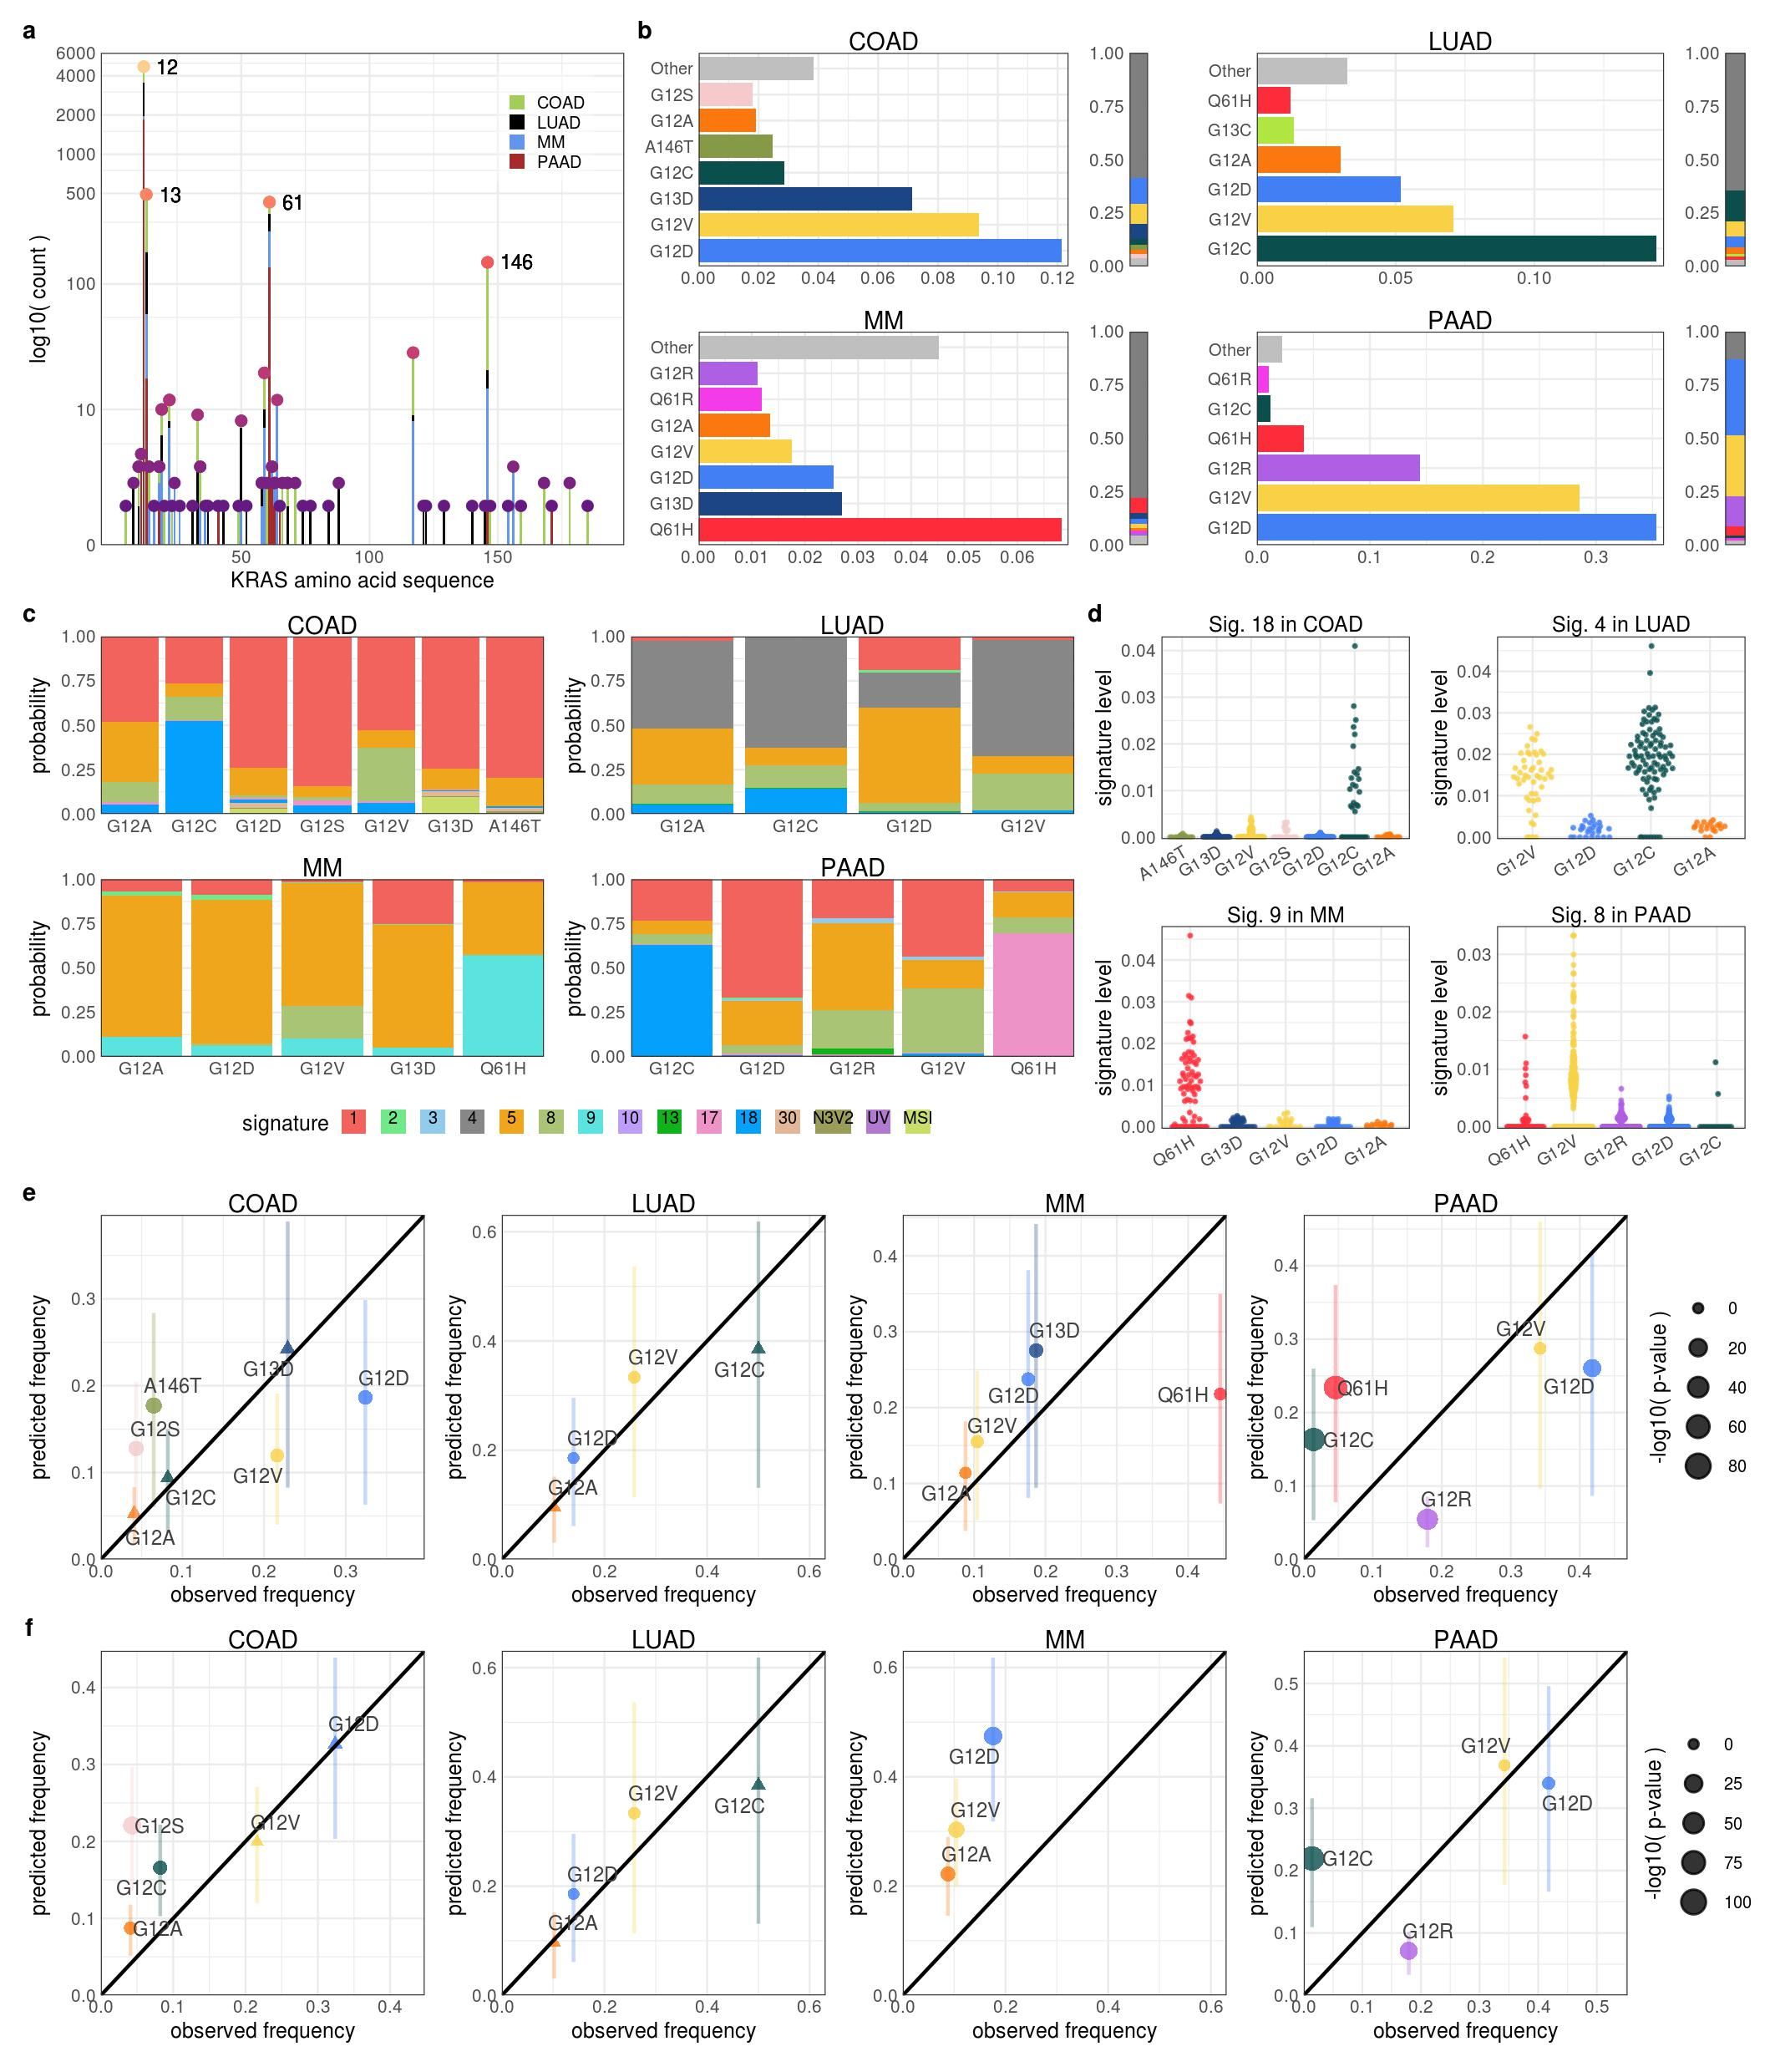
\includegraphics[height=160mm]{figures/Figure_01.jpeg}
\caption{
    \textbf{The contribution of mutational processes to \KRAS{} mutagenesis.}
    \textbf{a.} The number of samples with mutations along the \KRAS{} protein sequence. The most frequently mutated locations are labeled. The color of the bar indicates the abundance per cancer. 
    \textbf{b.} The distribution of \KRAS{} alleles in each cancer. The "Other" group includes the infrequent \KRAS{} alleles of the cancer. The adjacent bar indicates the fraction of samples with each \KRAS{} allele over all samples, including those with WT \KRAS{}.
    \textbf{c.} The average probability of each mutational signature to have caused the \KRAS{} mutation in a sample.
    \textbf{d.} The levels of select mutational signatures in samples with \KRAS{} mutations.
    \textbf{e, f.} The predicted vs. observed frequency of \KRAS{} alleles for all common alleles of the cancer (\textbf{e}) or only codon 12 alleles (\textbf{f}). $\blacktriangle$ indicate the failure to reject the null hypothesis that the observed and predicted frequencies are the same. Error bars indicate 95 \% confidence intervals of the predicted values.
}
\label{fig:mutational-signatures-main}
\end{figure}


\begin{figure}[p]
\centering
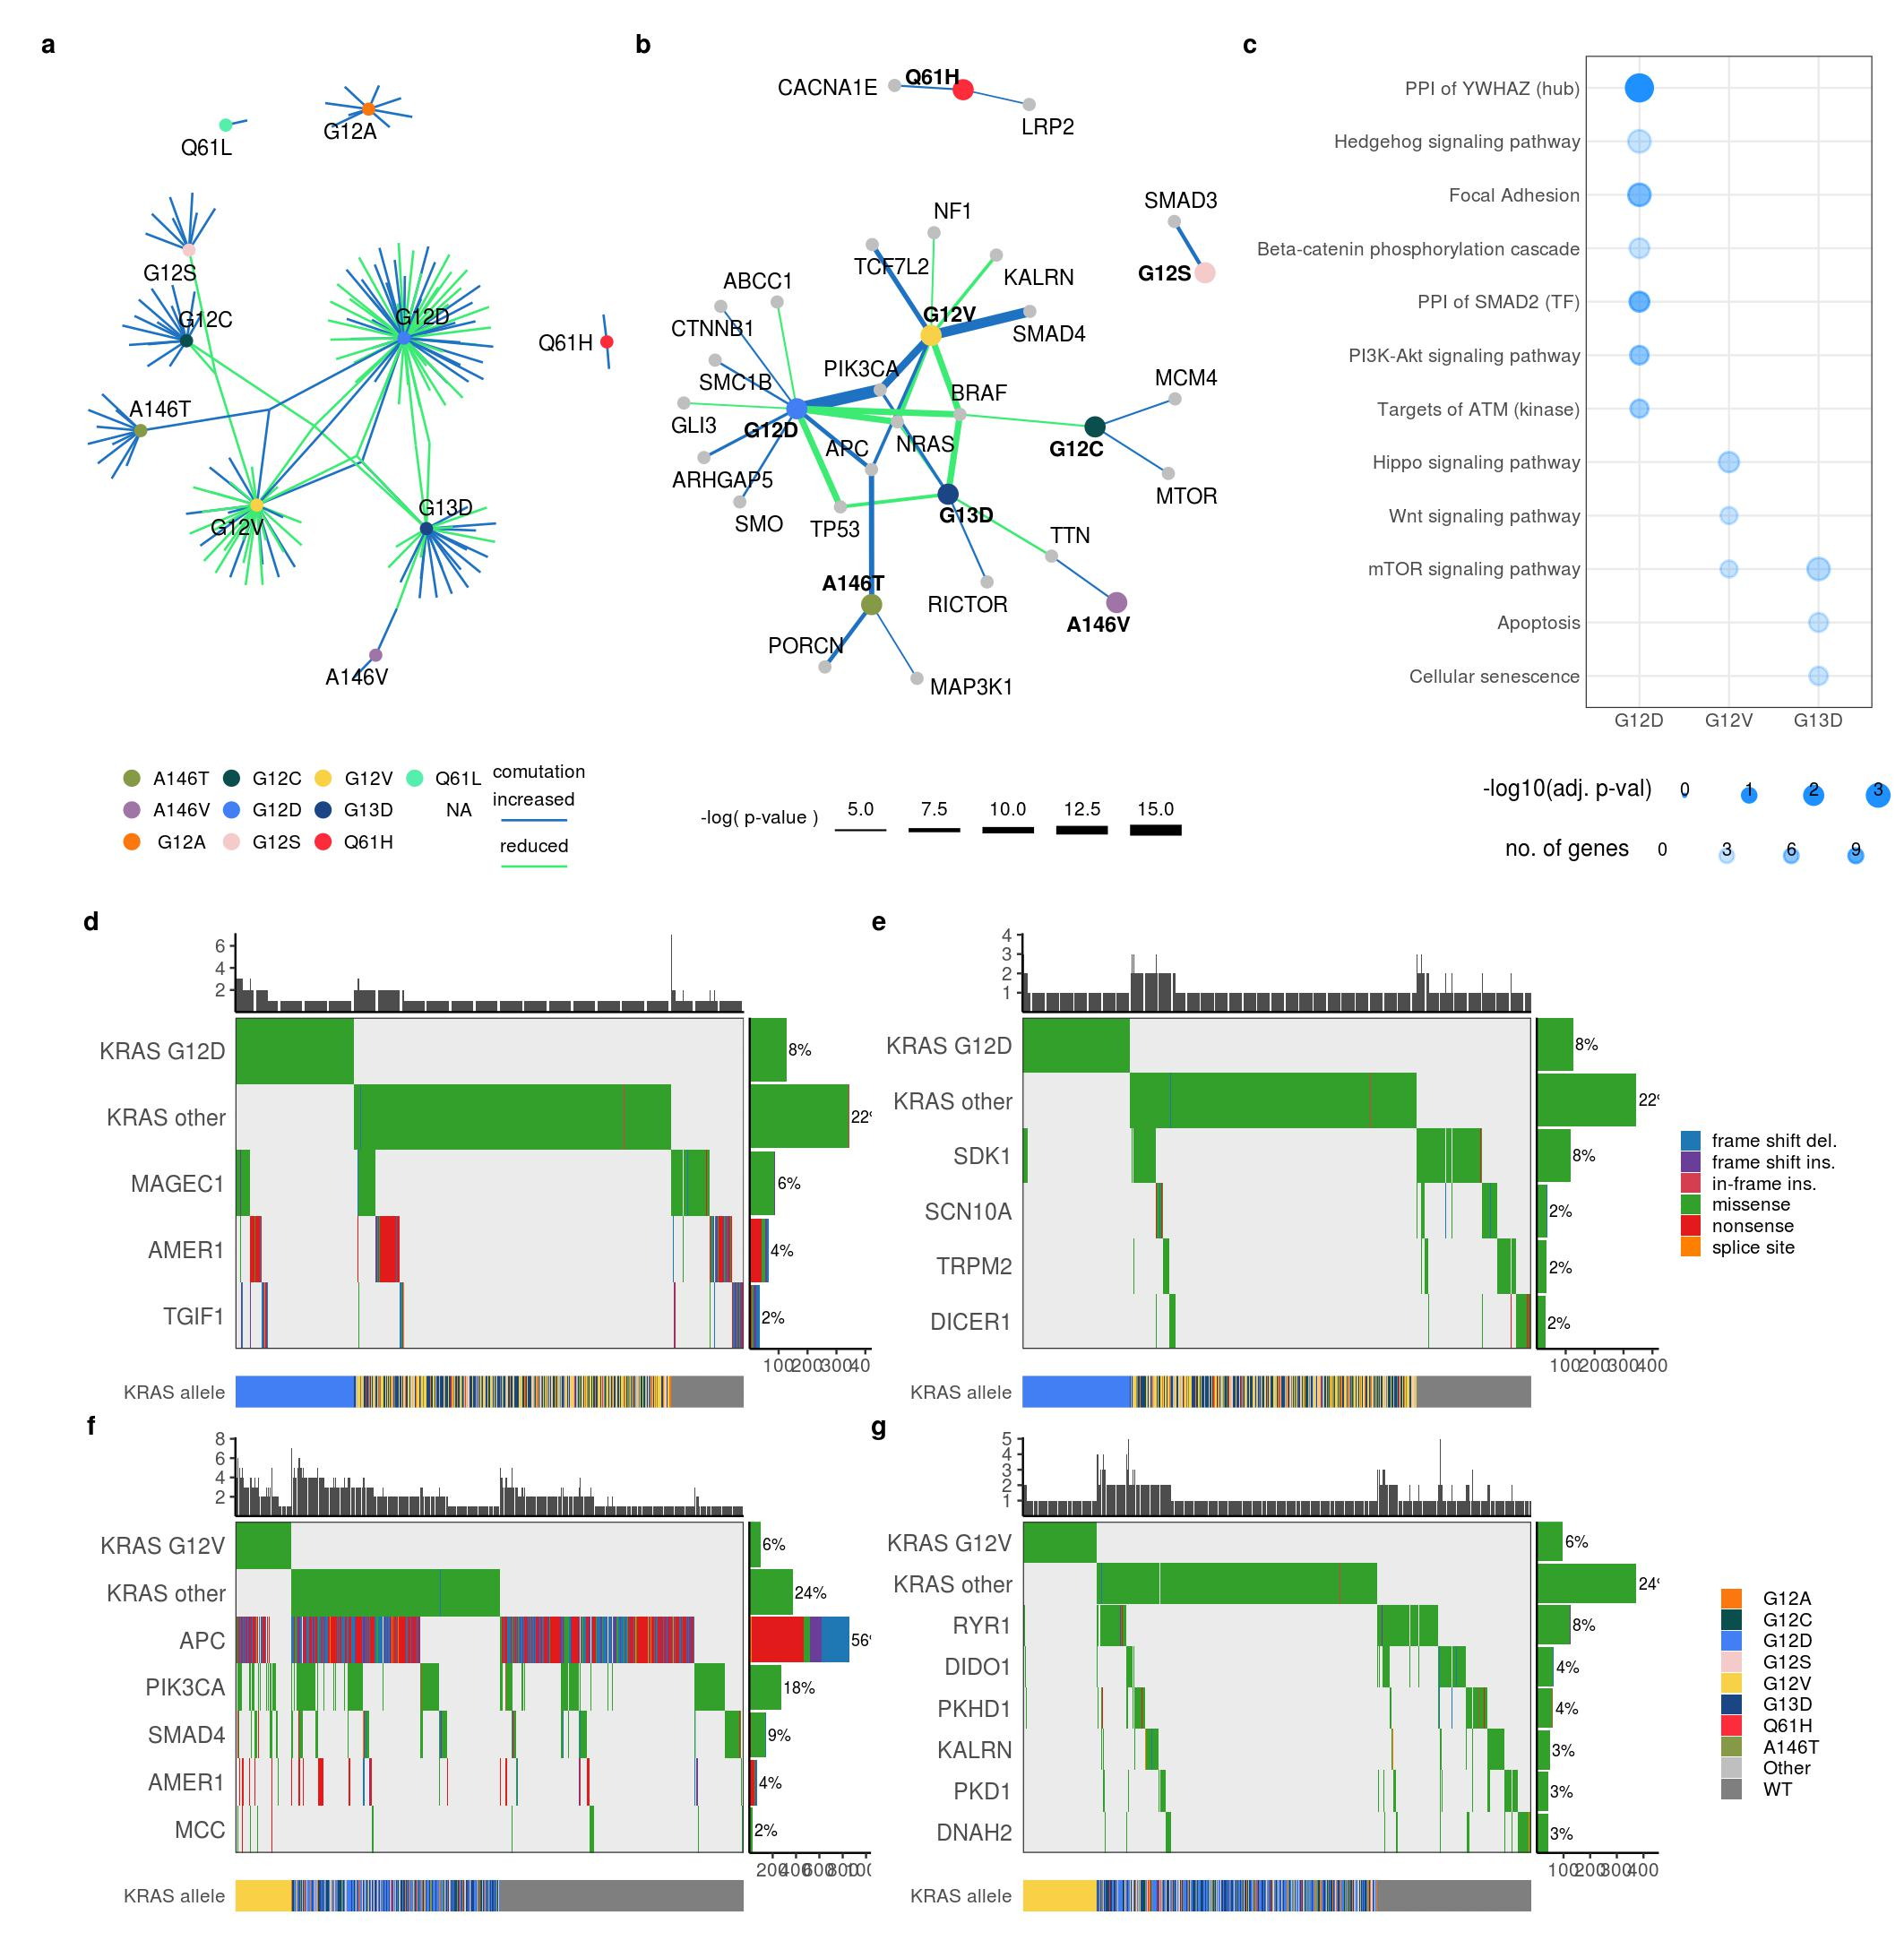
\includegraphics[height=135mm]{figures/Figure_02.jpeg}
\caption{
    \textbf{The comutation networks of common \KRAS{} alleles in COAD.}
    \textbf{a.} The comutation network of the \KRAS{} alleles in COAD with each edge representing a comutation interaction between an allele and another gene. The color of the edge indicates whether the interaction was an increase (blue) or decrease (green) in the frequency of comutation.
    \textbf{b.} A subset of the network shown in \textbf{a} of genes known to physically interact with \KRAS{}, are in one of its canonical up- or downstream pathways, or are validated oncogenes. The width of the edge indicates the strength of the association.
    \textbf{c.} Cellular functions enriched in the comutation networks of the \KRAS{} alleles. The size of the dot indicates the p-value of the enrichment and the transparency indicates the number of genes in both the function and the comutation network.
    \textbf{d, e, f, g.} A visualization of the increased (\textbf{d, f}) or decreased (\textbf{e, g}) comutation of select genes with \KRAS{} G12D (\textbf{d, e}) and G12V (\textbf{f, g}). Rows of the central plot represent genes. Each column of the central plot is a different tumor sample. A filled space denotes a mutation of the gene in the sample, the color describing the type of variant. The bar plots above and to the right indicate the marginal values of the central plot. The row below the central plot indicates the \KRAS{} alleles of the tumor samples in the central plot.
}
\label{fig:coad-comutation-main}
\end{figure}


\begin{figure}
\centering
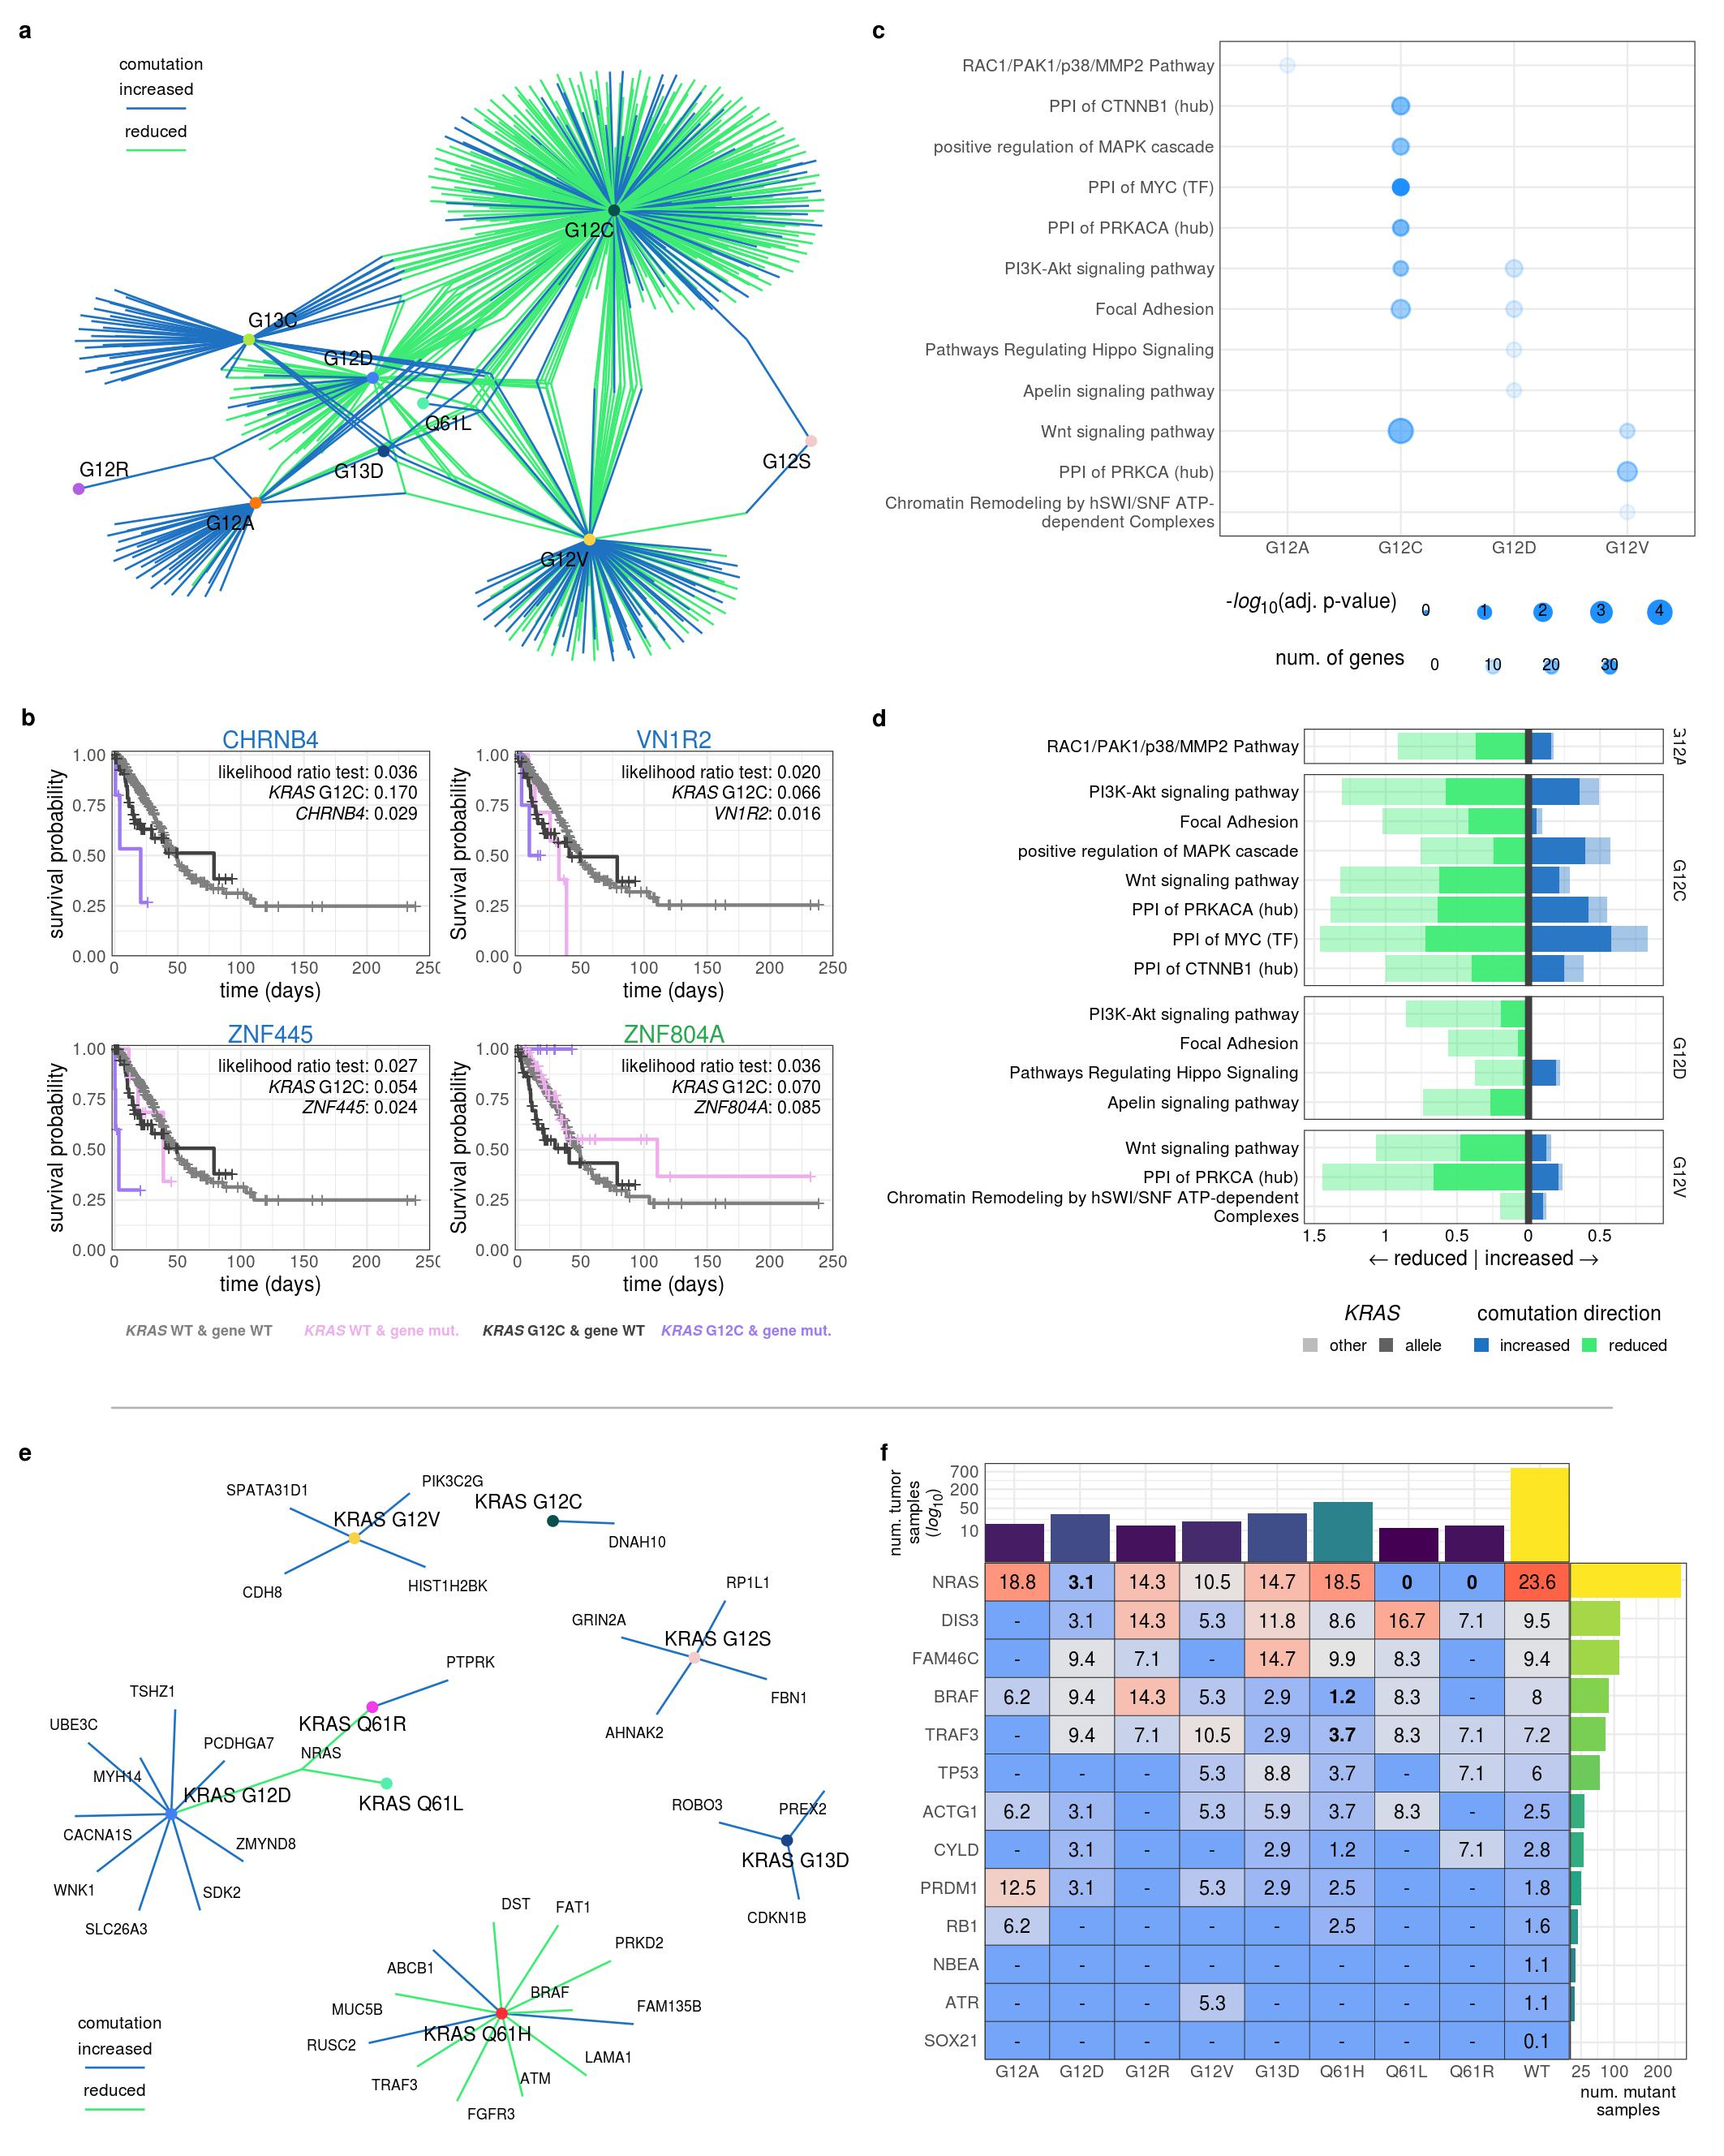
\includegraphics[height=130mm]{figures/Figure_03.jpeg}
\caption{
    \textbf{The comutation networks of \KRAS{} alleles in LUAD and MM.}
    \textbf{a.} The comutation network of the \KRAS{} alleles in LUAD where each edge represents a comutation interaction between an allele and another gene. The color of the edge indicates whether the interaction was an increase (blue) or decrease (green) in the frequency of comutation.
    \textbf{b.} Survival curves of patients with or without comutation of \KRAS{} G12C and a gene found to comutate with the allele (labeled above each plot). The color of the curve indicates the mutations of the tumor (grey: \KRAS{} and the other gene are WT; black: \KRAS{} G12C; pink: the other gene is mutated; purple: both \KRAS{} G12C and the other gene is mutated). The p-values for the likelihood ratio test and the regression covariates for the \KRAS{} G12C allele and the other gene are indicated on the plot.
    \textbf{c.} Cellular functions enriched in the comutation networks of the \KRAS{} alleles. The size of the dot indicates the p-value of the enrichment and the transparency indicates the number of genes in both the function and the comutation network.
    \textbf{d.} The combined rate of comutation of the genes underlying the enriched functions shown in \textbf{b}. The x-axis indicates the fraction of samples with at least one of the interacting genes mutated in the samples with the indicated \KRAS{} allele (dark) or the other samples (light). The genes were separated into those with an increase (blue, going right) or a reduced (green, going left) rate of comutation with the \KRAS{} allele.
    \textbf{e.} Each edge represents a comutation interaction between an allele and the indicated gene. The color of the edge indicates whether the interaction was an increase (blue) or decrease (green) in the frequency of comutation.
    \textbf{f.} A heatmap of the comutation frequencies between known MM driving genes and \KRAS{} alleles. The color is correlated with the comutation frequency, indicated in each cell. Bold percent values indicate statistical significance of a comutation interaction (see Methods). The bar plot along the top indicates the number of samples with the \KRAS{} allele, and the bar plot on the right indicates the number of samples with a mutation in the gene.
}
\label{fig:luadmm-comutation-main}
\end{figure}


\begin{figure}
\centering
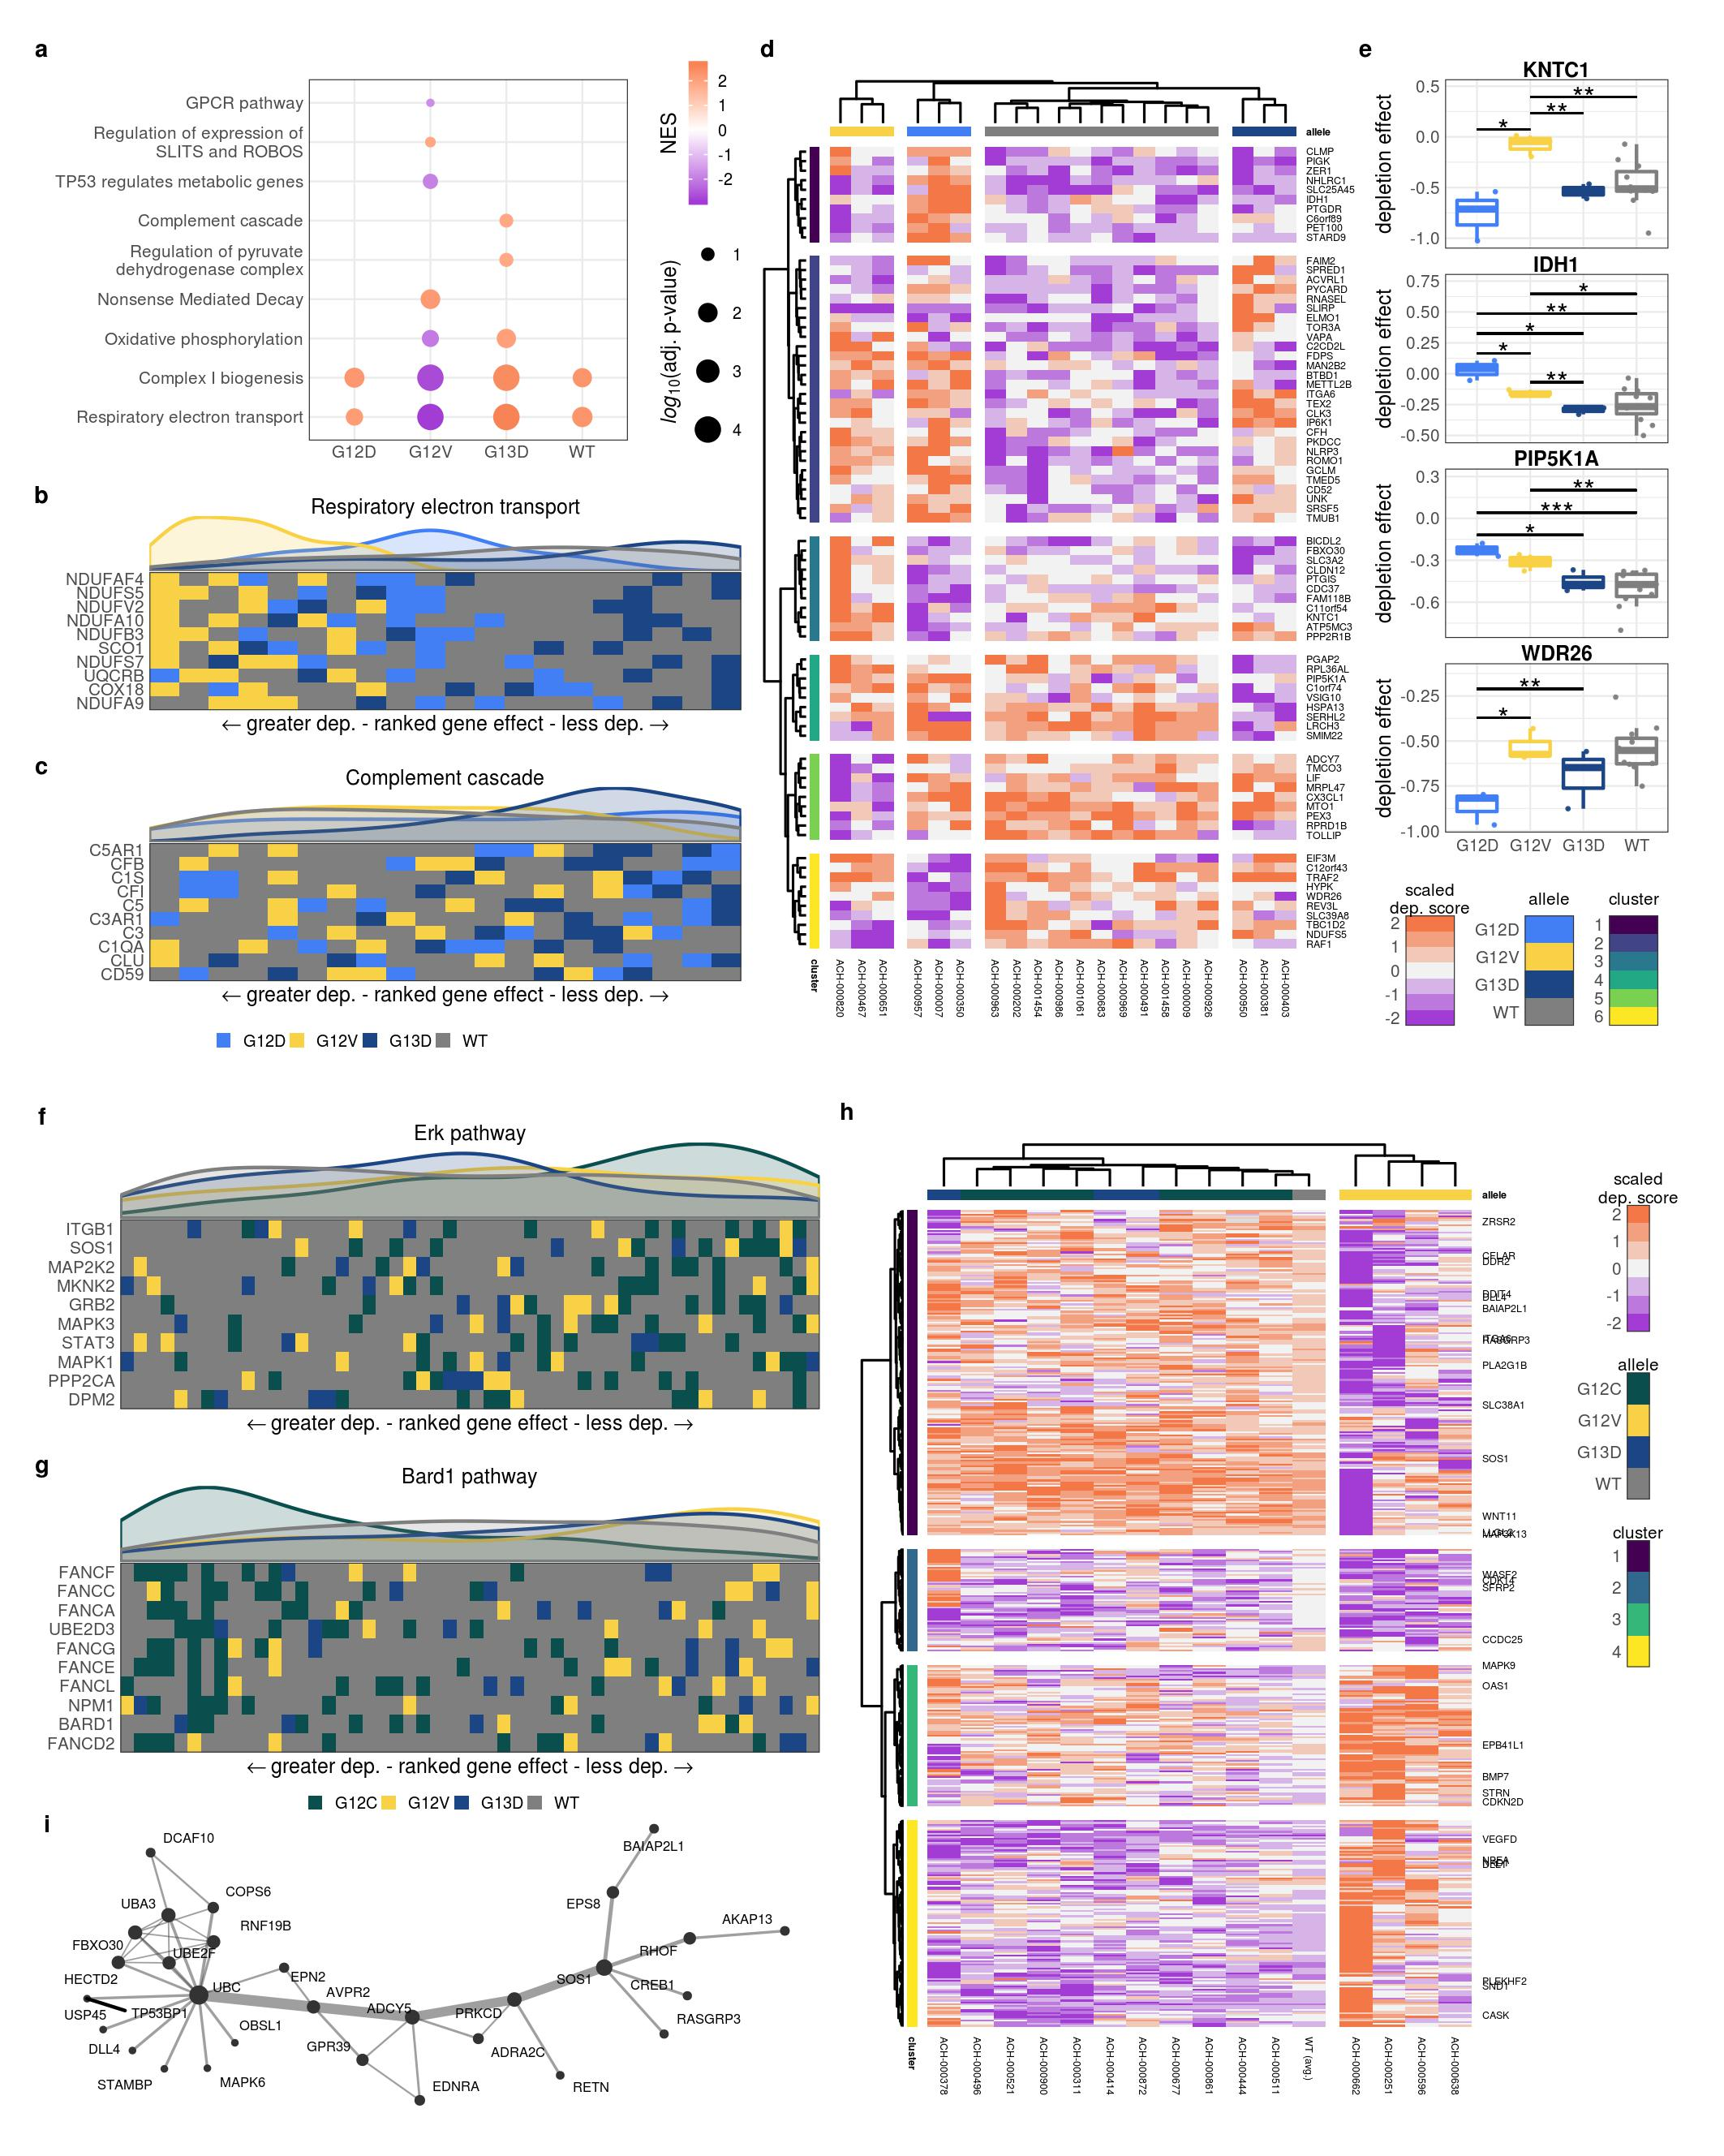
\includegraphics[height=150mm]{figures/Figure_04.jpeg}
\caption{
    \textbf{Allele-specific genetic dependencies in COAD and LUAD cell lines.}
    \textbf{a.} Gene sets with significant enrichment for increased (lower dependency score; purple) or reduced (higher dependency score; orange) genetic dependency in COAD cell lines. The size of the dot relates the p-value of the association and the color indicated the strength of the enrichment ("normalized enrichment score").
    \textbf{b, c, f, g.} Heatmaps ranking the cell lines by dependency score of the genes at the leading edge of enrichment for two gene sets in COAD (\textbf{b}, \textbf{c}) and two enriched gene sets in LUAD cell lines (\textbf{f}, \textbf{g}). Each row represents a gene and each cell represents a cell line colored by its \KRAS{} allele. The cell lines were arranged in ranking order by their dependency score for the gene. Thus, each column indicates a rank. The line plots above the heatmaps indicate the representation (density) of each \KRAS{} allele at each rank across the genes.
    \textbf{d, h.} Clustered heatmaps of the genes that demonstrated differential genetic dependency amongst cell lines of different \KRAS{} alleles in COAD (\textbf{d}) or LUAD (\textbf{h}) cell lines. Each column is a cell line labeled by its DepMap ID and each row is a gene. For \textbf{h}, only genes known to be involved in \KRAS{} signaling or previously implicated in driving cancer are labeled. Also, for visualization purposes, the scores of the WT cell lines were averaged into a single, representative group, labeled "WT (avg.)."
    \textbf{e.} Examples of genes that demonstrated differential genetic dependency amongst cell lines of different \KRAS{} alleles in COAD (*: p < 0.05, **: p < 0.01, ***: p < 0.001; p-values were adjusted using the Benjamini-Hochberg FDR correction method).
    \textbf{i.} A PPI comprised of proteins whose genes were in cluster 4 of the deferentially dependent genes in LUAD cell lines (\textbf{h}).
}
\label{fig:coadluad-dependency-main}
\end{figure}


\begin{figure}
\centering
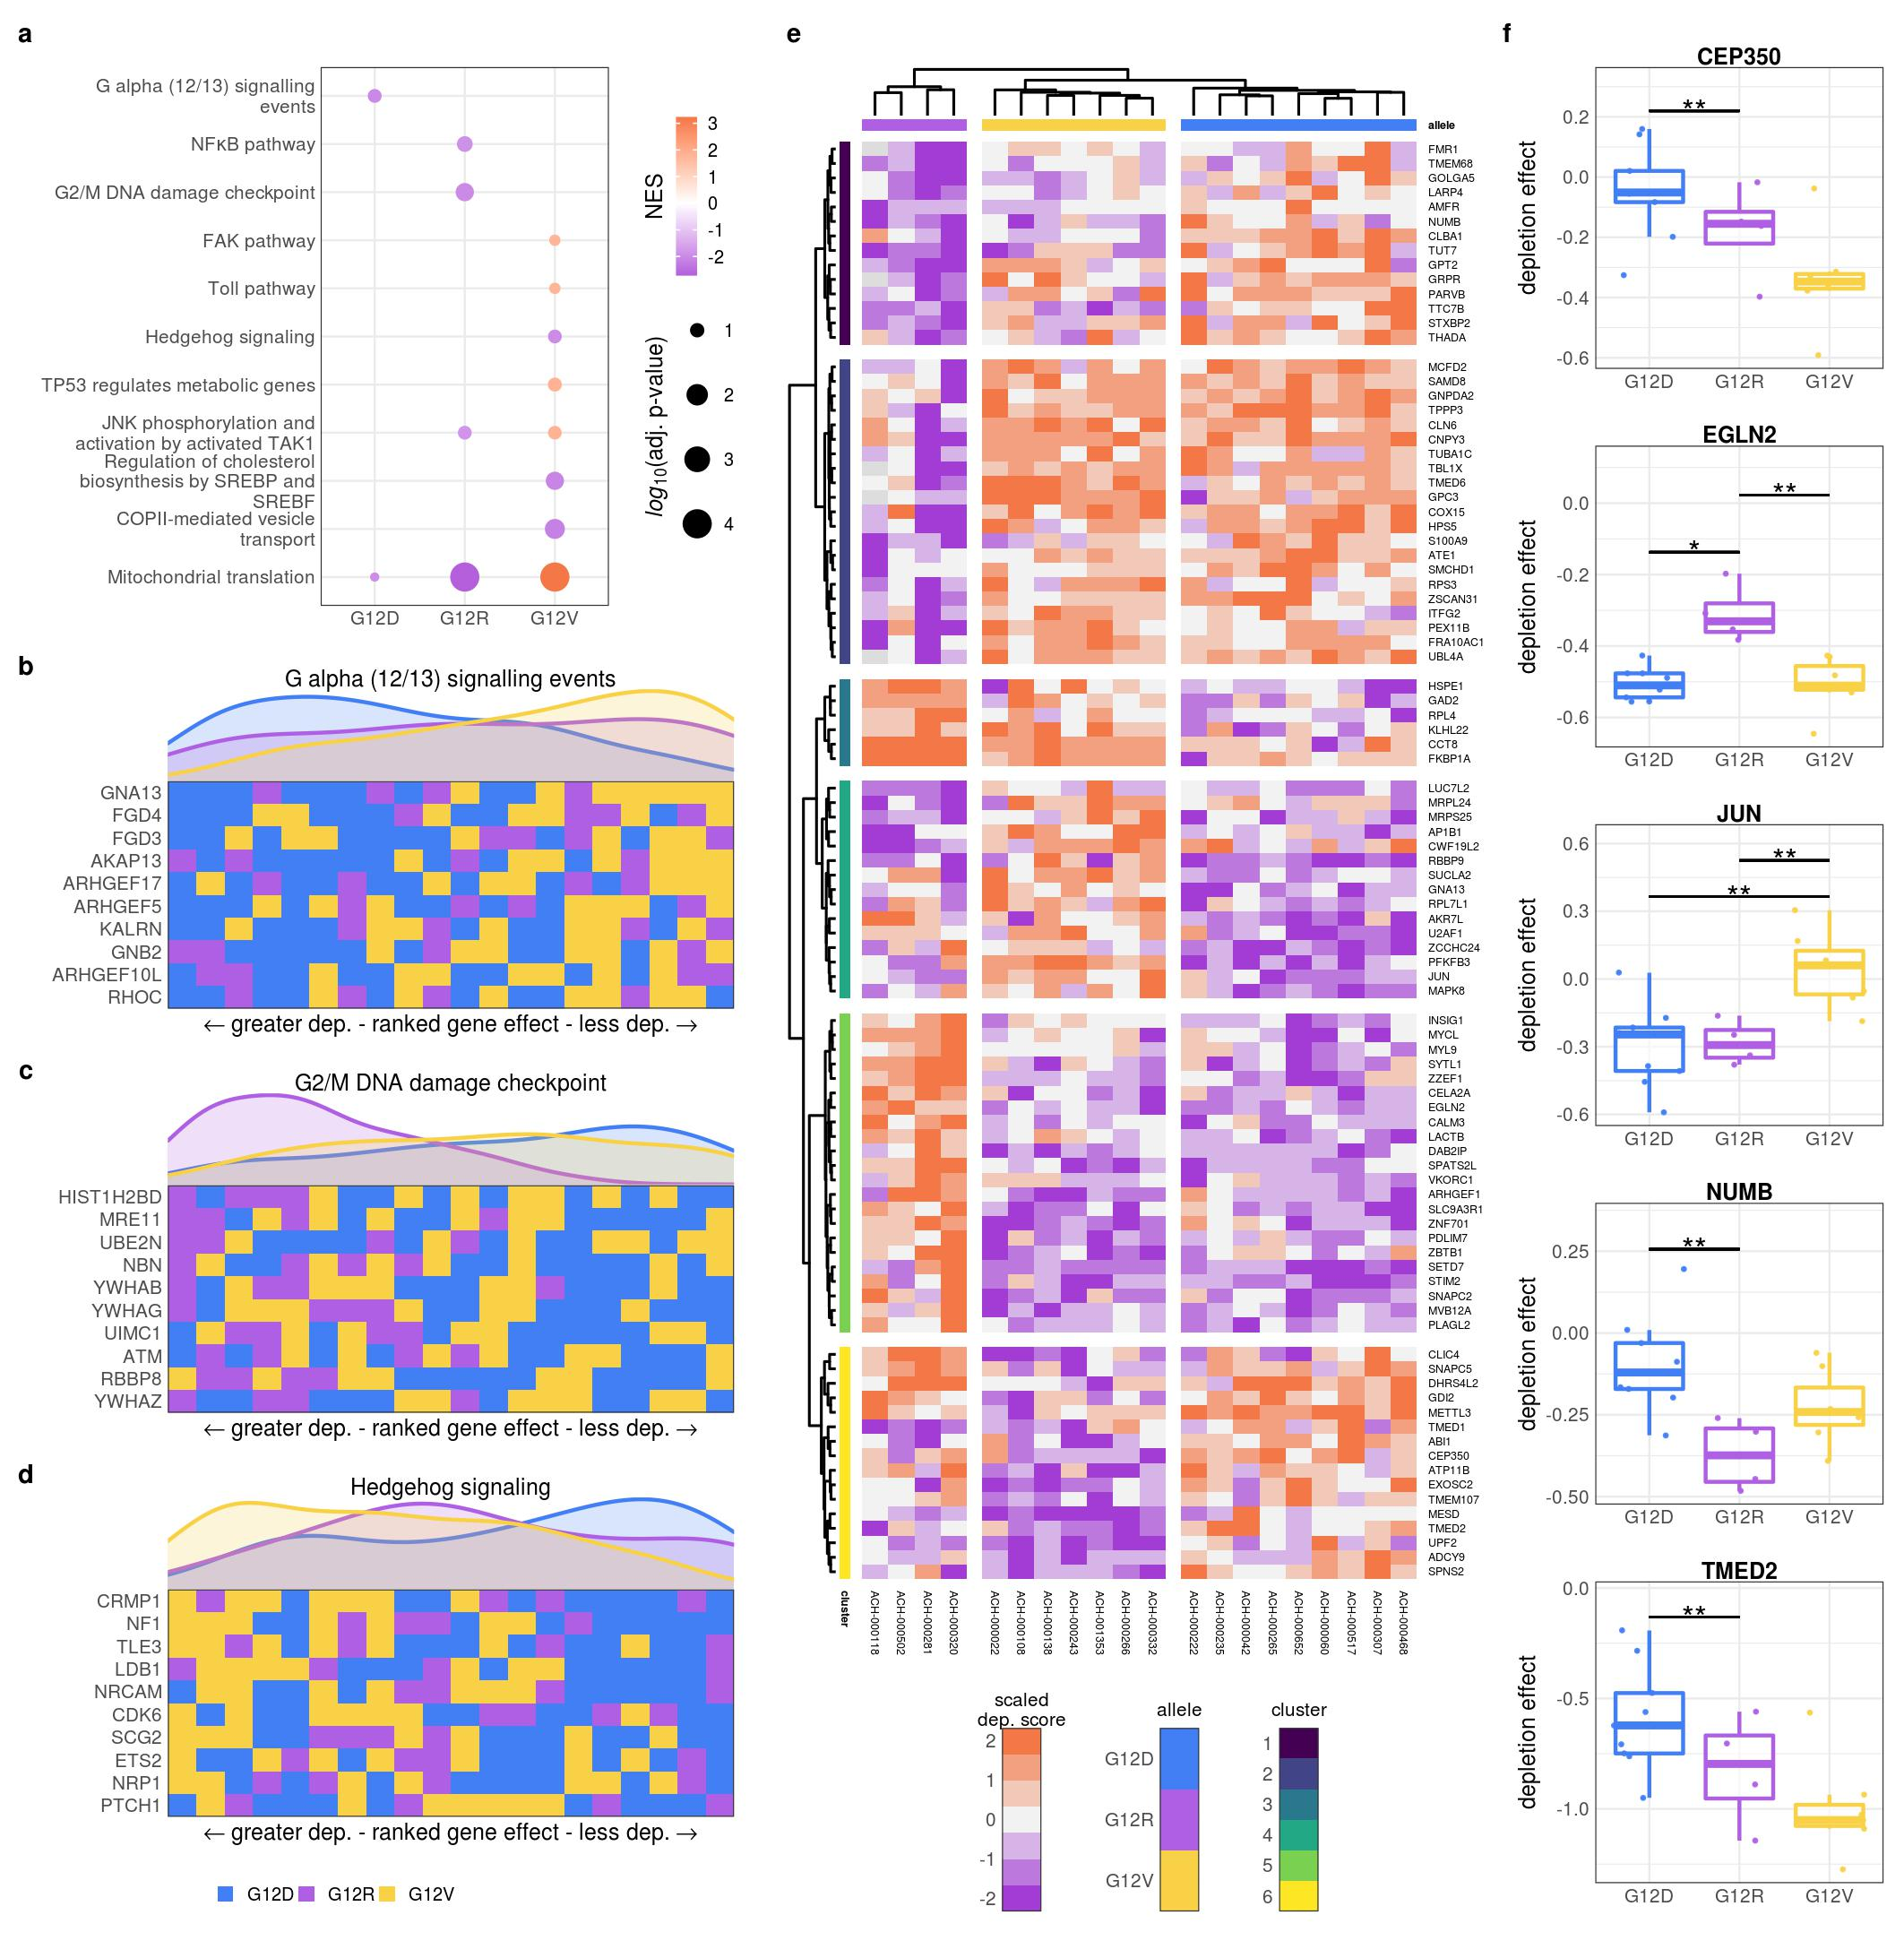
\includegraphics[height=145mm]{figures/SuppFigure_13.jpeg}
\caption{
    \textbf{Allele-specific genetic dependencies in PAAD cell lines.}
    \textbf{a.} Gene sets with significant enrichment for increased (lower dependency score; purple) or reduced (higher dependency score; orange) genetic dependency in PAAD cell lines. The size of the dot relates the p-value of the association and the color indicated the strength of the enrichment.
    \textbf{b, c, d.} Heatmaps ranking the cell lines by dependency score of genes at the leading edge of enrichment for three gene sets in PAAD. Each row represents a gene and each cell represents a cell line colored by its \KRAS{} allele. The cell lines were arranged in ranking order by their dependency score for the gene. Thus, each column indicates a rank. The line plots above the heatmaps indicate the representation (density) of each \KRAS{} allele at each rank across the genes.
    \textbf{e.} Clustered heatmaps of the genes that demonstrated differential genetic dependency amongst cell lines of different \KRAS{} alleles in PAAD cell lines. Each column is a cell line labeled by its DepMap ID and each row is a gene.
    \textbf{f.} Examples of genes that demonstrated differential genetic dependency amongst cell lines of different \KRAS{} alleles in PAAD (*: p < 0.05, **: p < 0.01, ***: p < 0.001; p-values were adjusted using the Benjamini-Hochberg FDR correction method).
}
\label{fig:paad-dependency-main}
\end{figure}


\begin{figure}
\centering
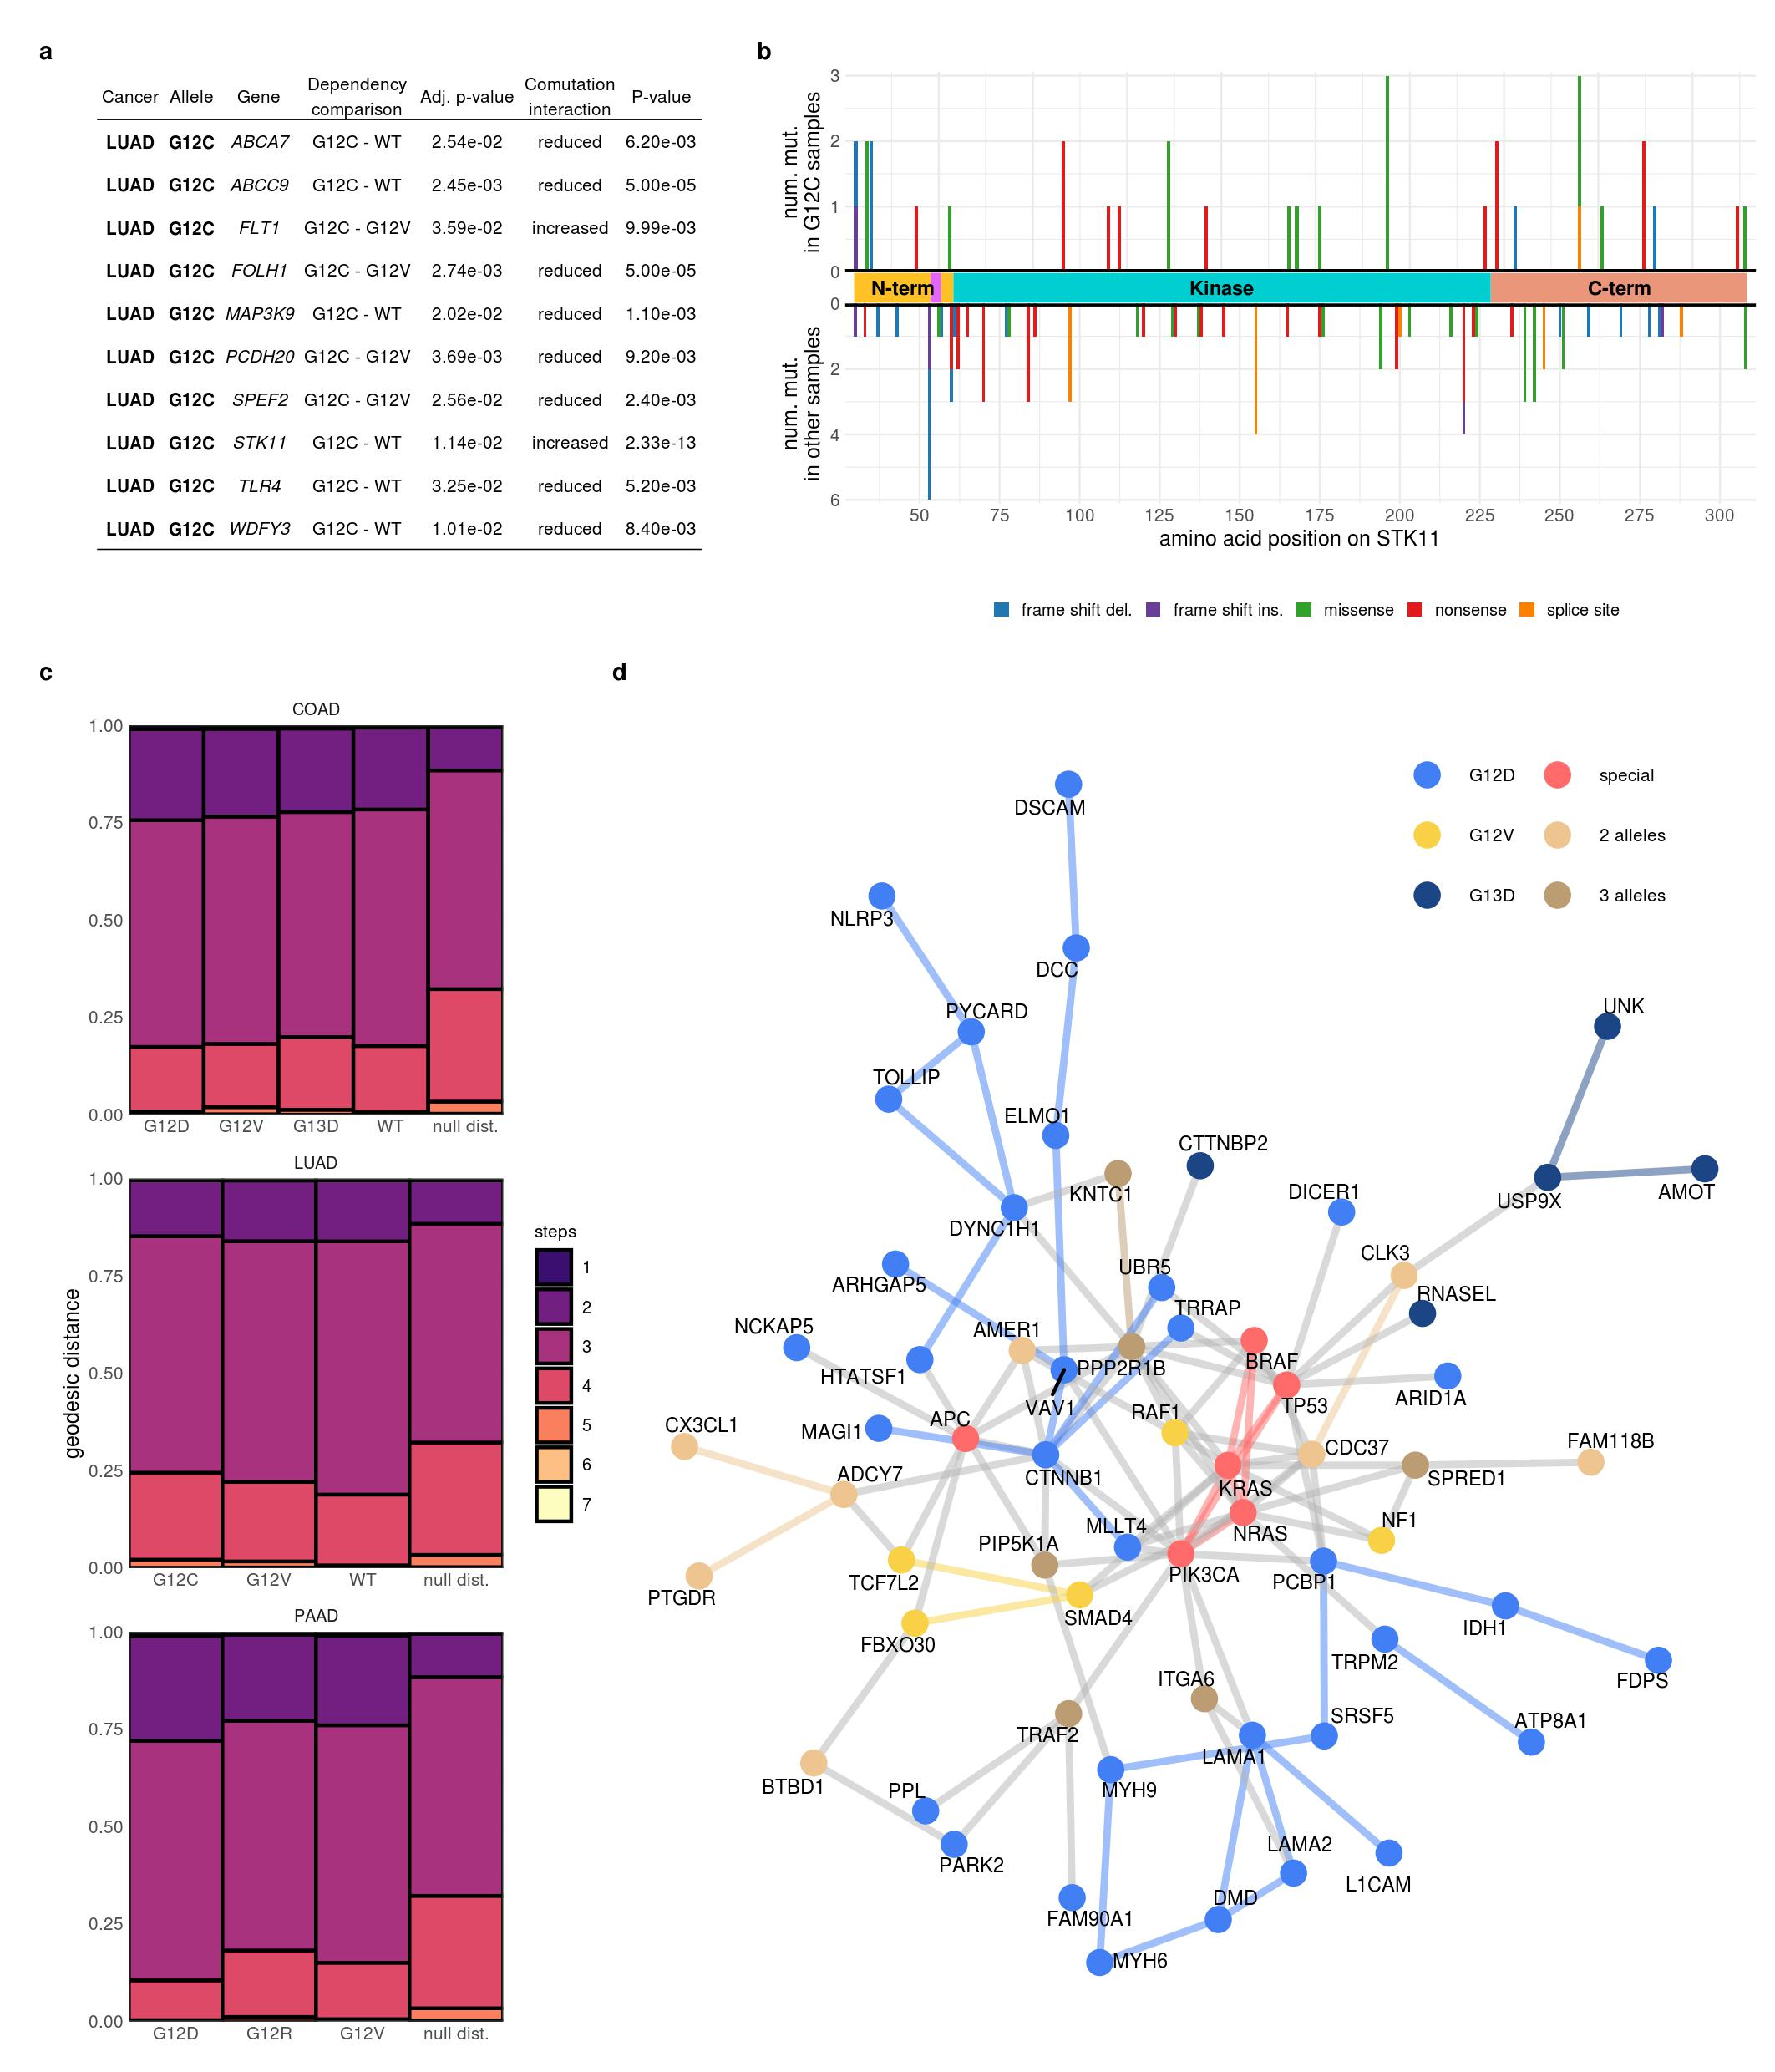
\includegraphics[height=100mm]{figures/Figure_05.jpeg}
\caption{
    \textbf{Integration of comutation and genetic dependency results.}
    \textbf{a.} A table of the genes found to comutate and demonstrate differential dependency with the same \KRAS{} allele. The "Dependency comparison" indicates the comparison of dependency scores found to be statistically significant; the "Adj. p-value" is the Benjamini-Hochberg-adjusted p-value for the comparison. The "Comutation interaction" indicates if the comutation interaction was a reduced or increased rate of comutation; the "P-value" is the p-value for this interaction.
    \textbf{b.} The mutations along STK11 separated by those in \KRAS{} G12C-mutant samples (top) and the rest of the samples (bottom). The color of the vertical bars indicates the type of mutation, and a red dot at the top indicates if missense mutations at the location are predicted or known to be functionally damaging. The domains of STK11 are shown between the bar-plots. The magenta portion of the N-terminus is the nuclear localization signal.
    \textbf{c.} The connectivity of the proteins encoded by the genes found to comutate or demonstrate differential dependence with each \KRAS{} allele on the PPIN. The right-most column represents the null distribution of the connectivity of randomly selected pairs of nodes. The bars indicate the distribution of the geodesic distances (shortest path length) between nodes in the PPIN.
    \textbf{d.} The largest connected subnetwork of the PPIN of genes found to comutate or demonstrate differential dependence with each \KRAS{} allele was extracted. The network shown is the overlap of the subnetworks for each \KRAS{} allele in COAD. Nodes present in multiple subnetworks are colored shades of brown, save for prominent oncogenes and tumor suppressors in COAD, shown in red ("special"). The rest of the nodes are colored by which allele they are associated with. The edges share the color of the nodes they connect if the nodes are the same color, otherwise are grey.
}
\label{fig:results_integration_main}
\end{figure}



\beginsupplement



\begin{figure}[p]
\centering
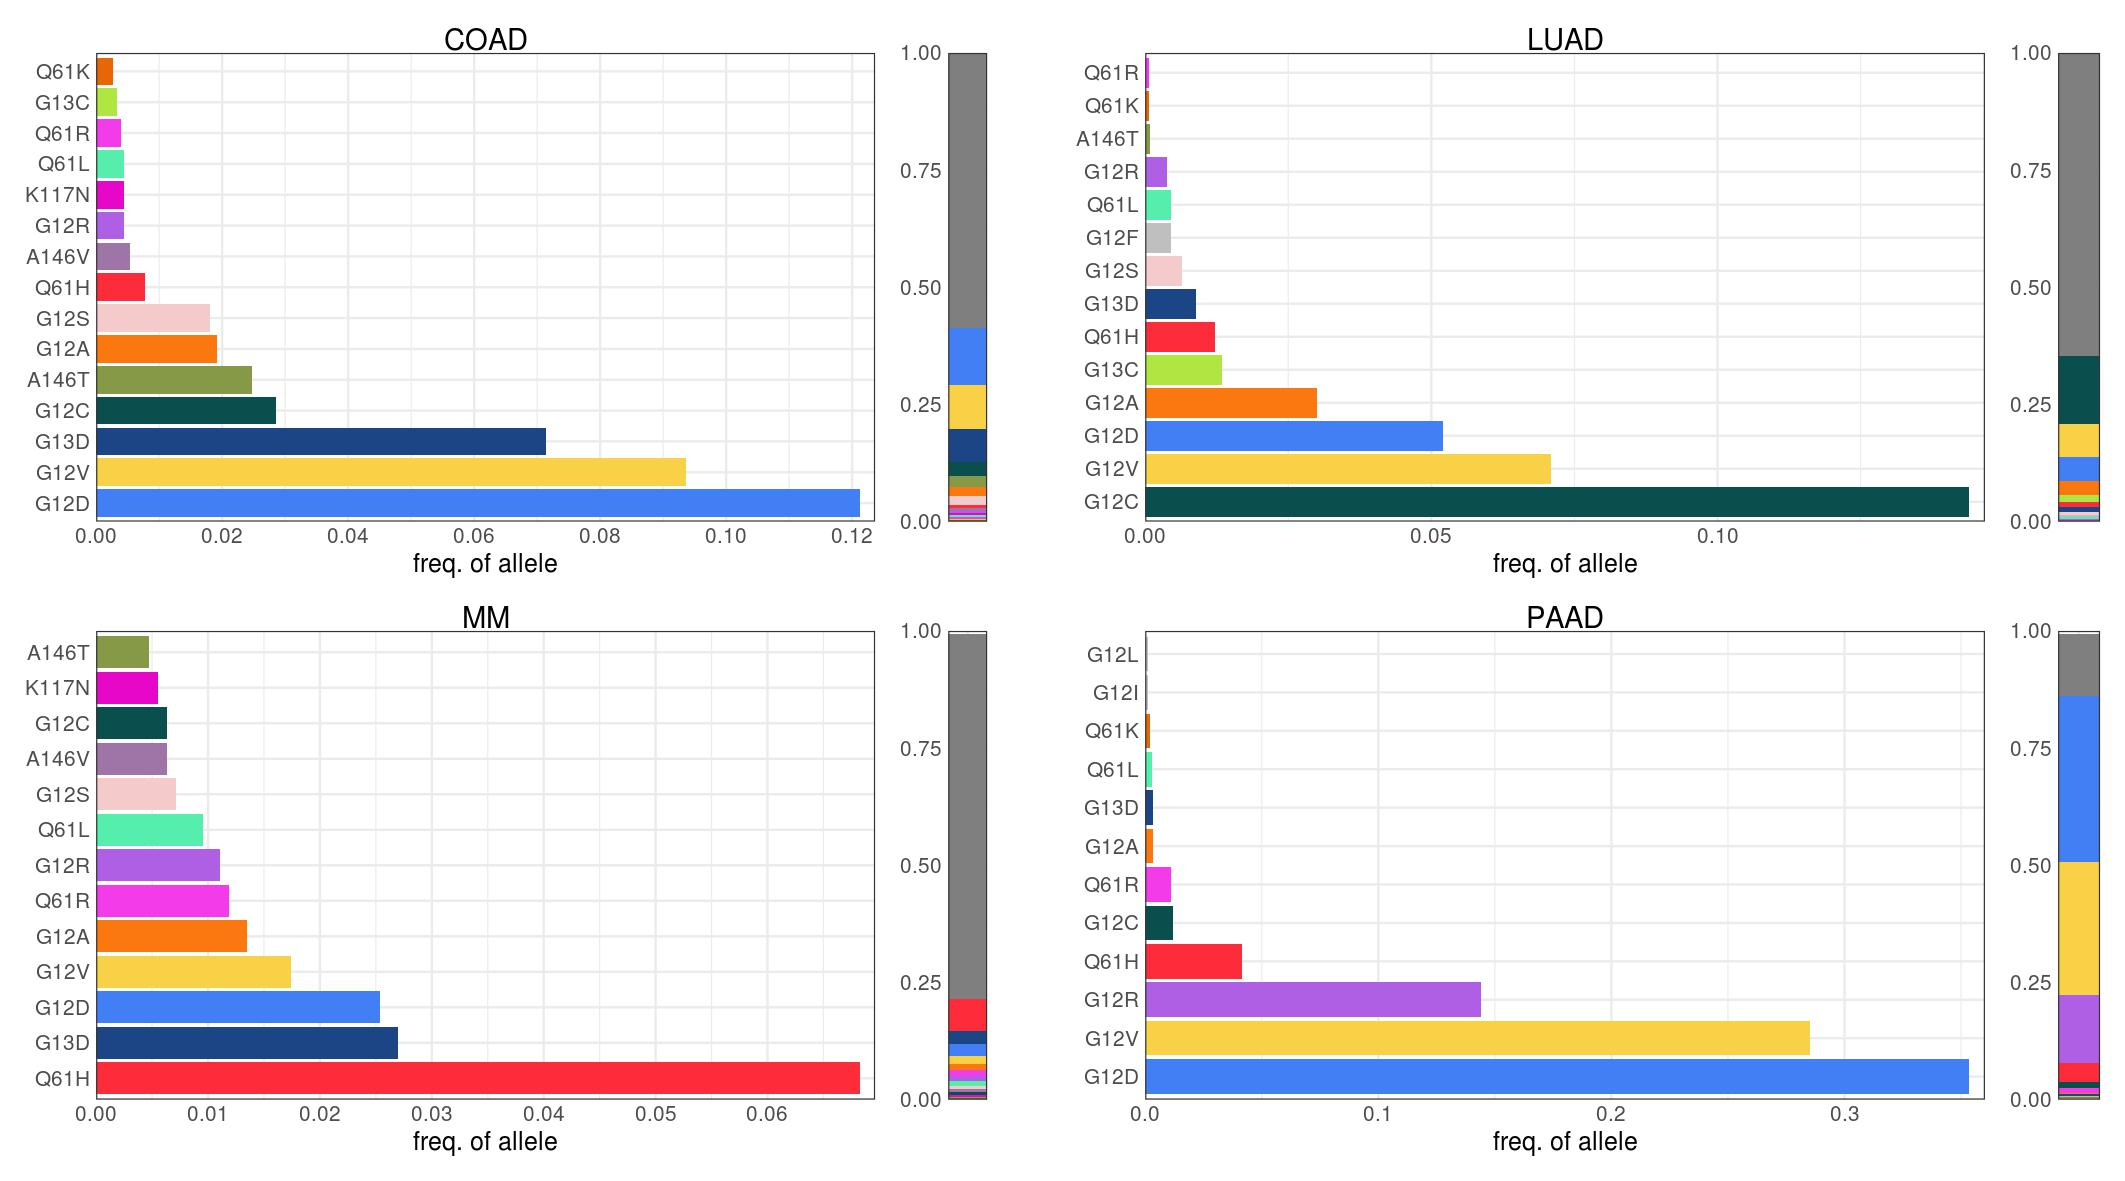
\includegraphics[width=\textwidth]{figures/SuppFigure_01.jpeg}
\caption{
    \textbf{The complete distribution of \KRAS{} alleles in each cancer.} The adjacent bar indicates the fraction of samples with each \KRAS{} allele over all samples, including those with WT \KRAS{}.
}
\label{sfig:expanded-kras-allele-distribution}
\end{figure}


\begin{figure}[p]
\centering
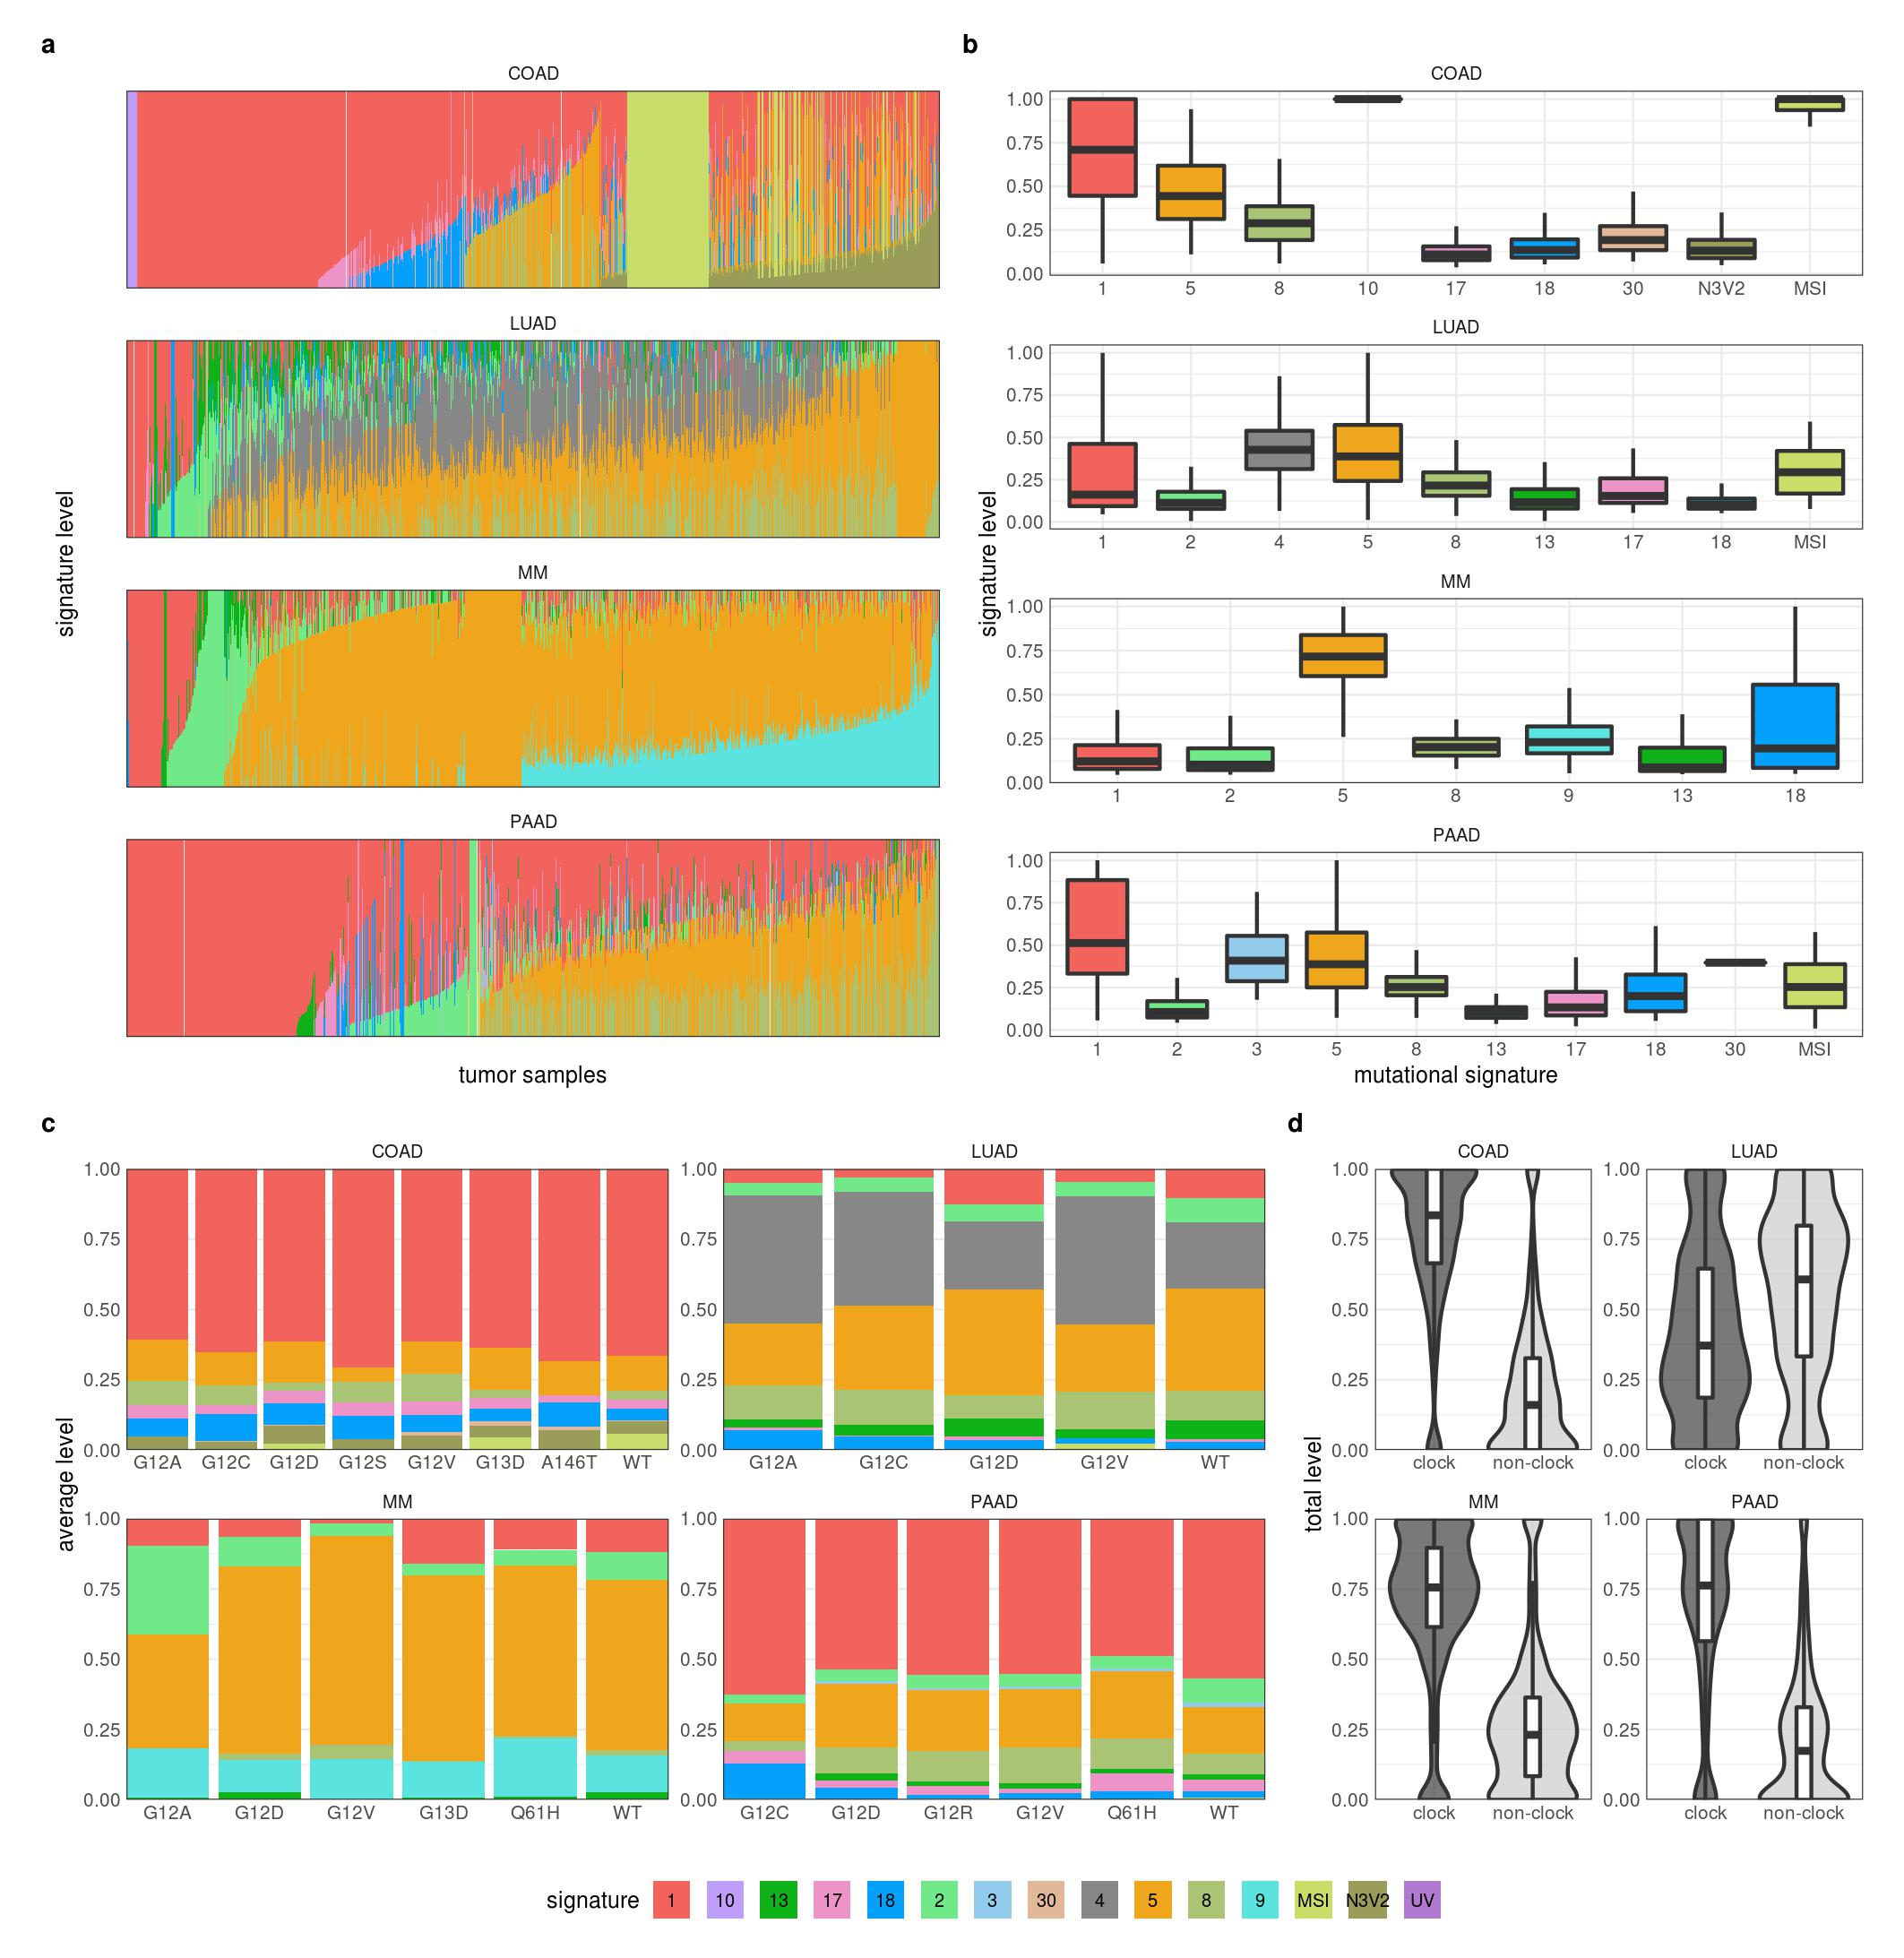
\includegraphics[height=160mm]{figures/SuppFigure_02.jpeg}
\caption{
    \textbf{Mutational signatures in tumor samples.}
    \textbf{a, b.} The detected level of the mutational signatures in each tumor sample. In \textbf{a}, each tumor sample is a column.
    \textbf{c.} The average levels of mutational signatures in samples separated by \KRAS{} allele.
    \textbf{d.} The average levels of clock (signatures 1 and 5) and non-clock (all other signatures) in the tumor samples.
}
\label{sfig:mutational-signatures-summary}
\end{figure}


\begin{figure}[p]
\centering
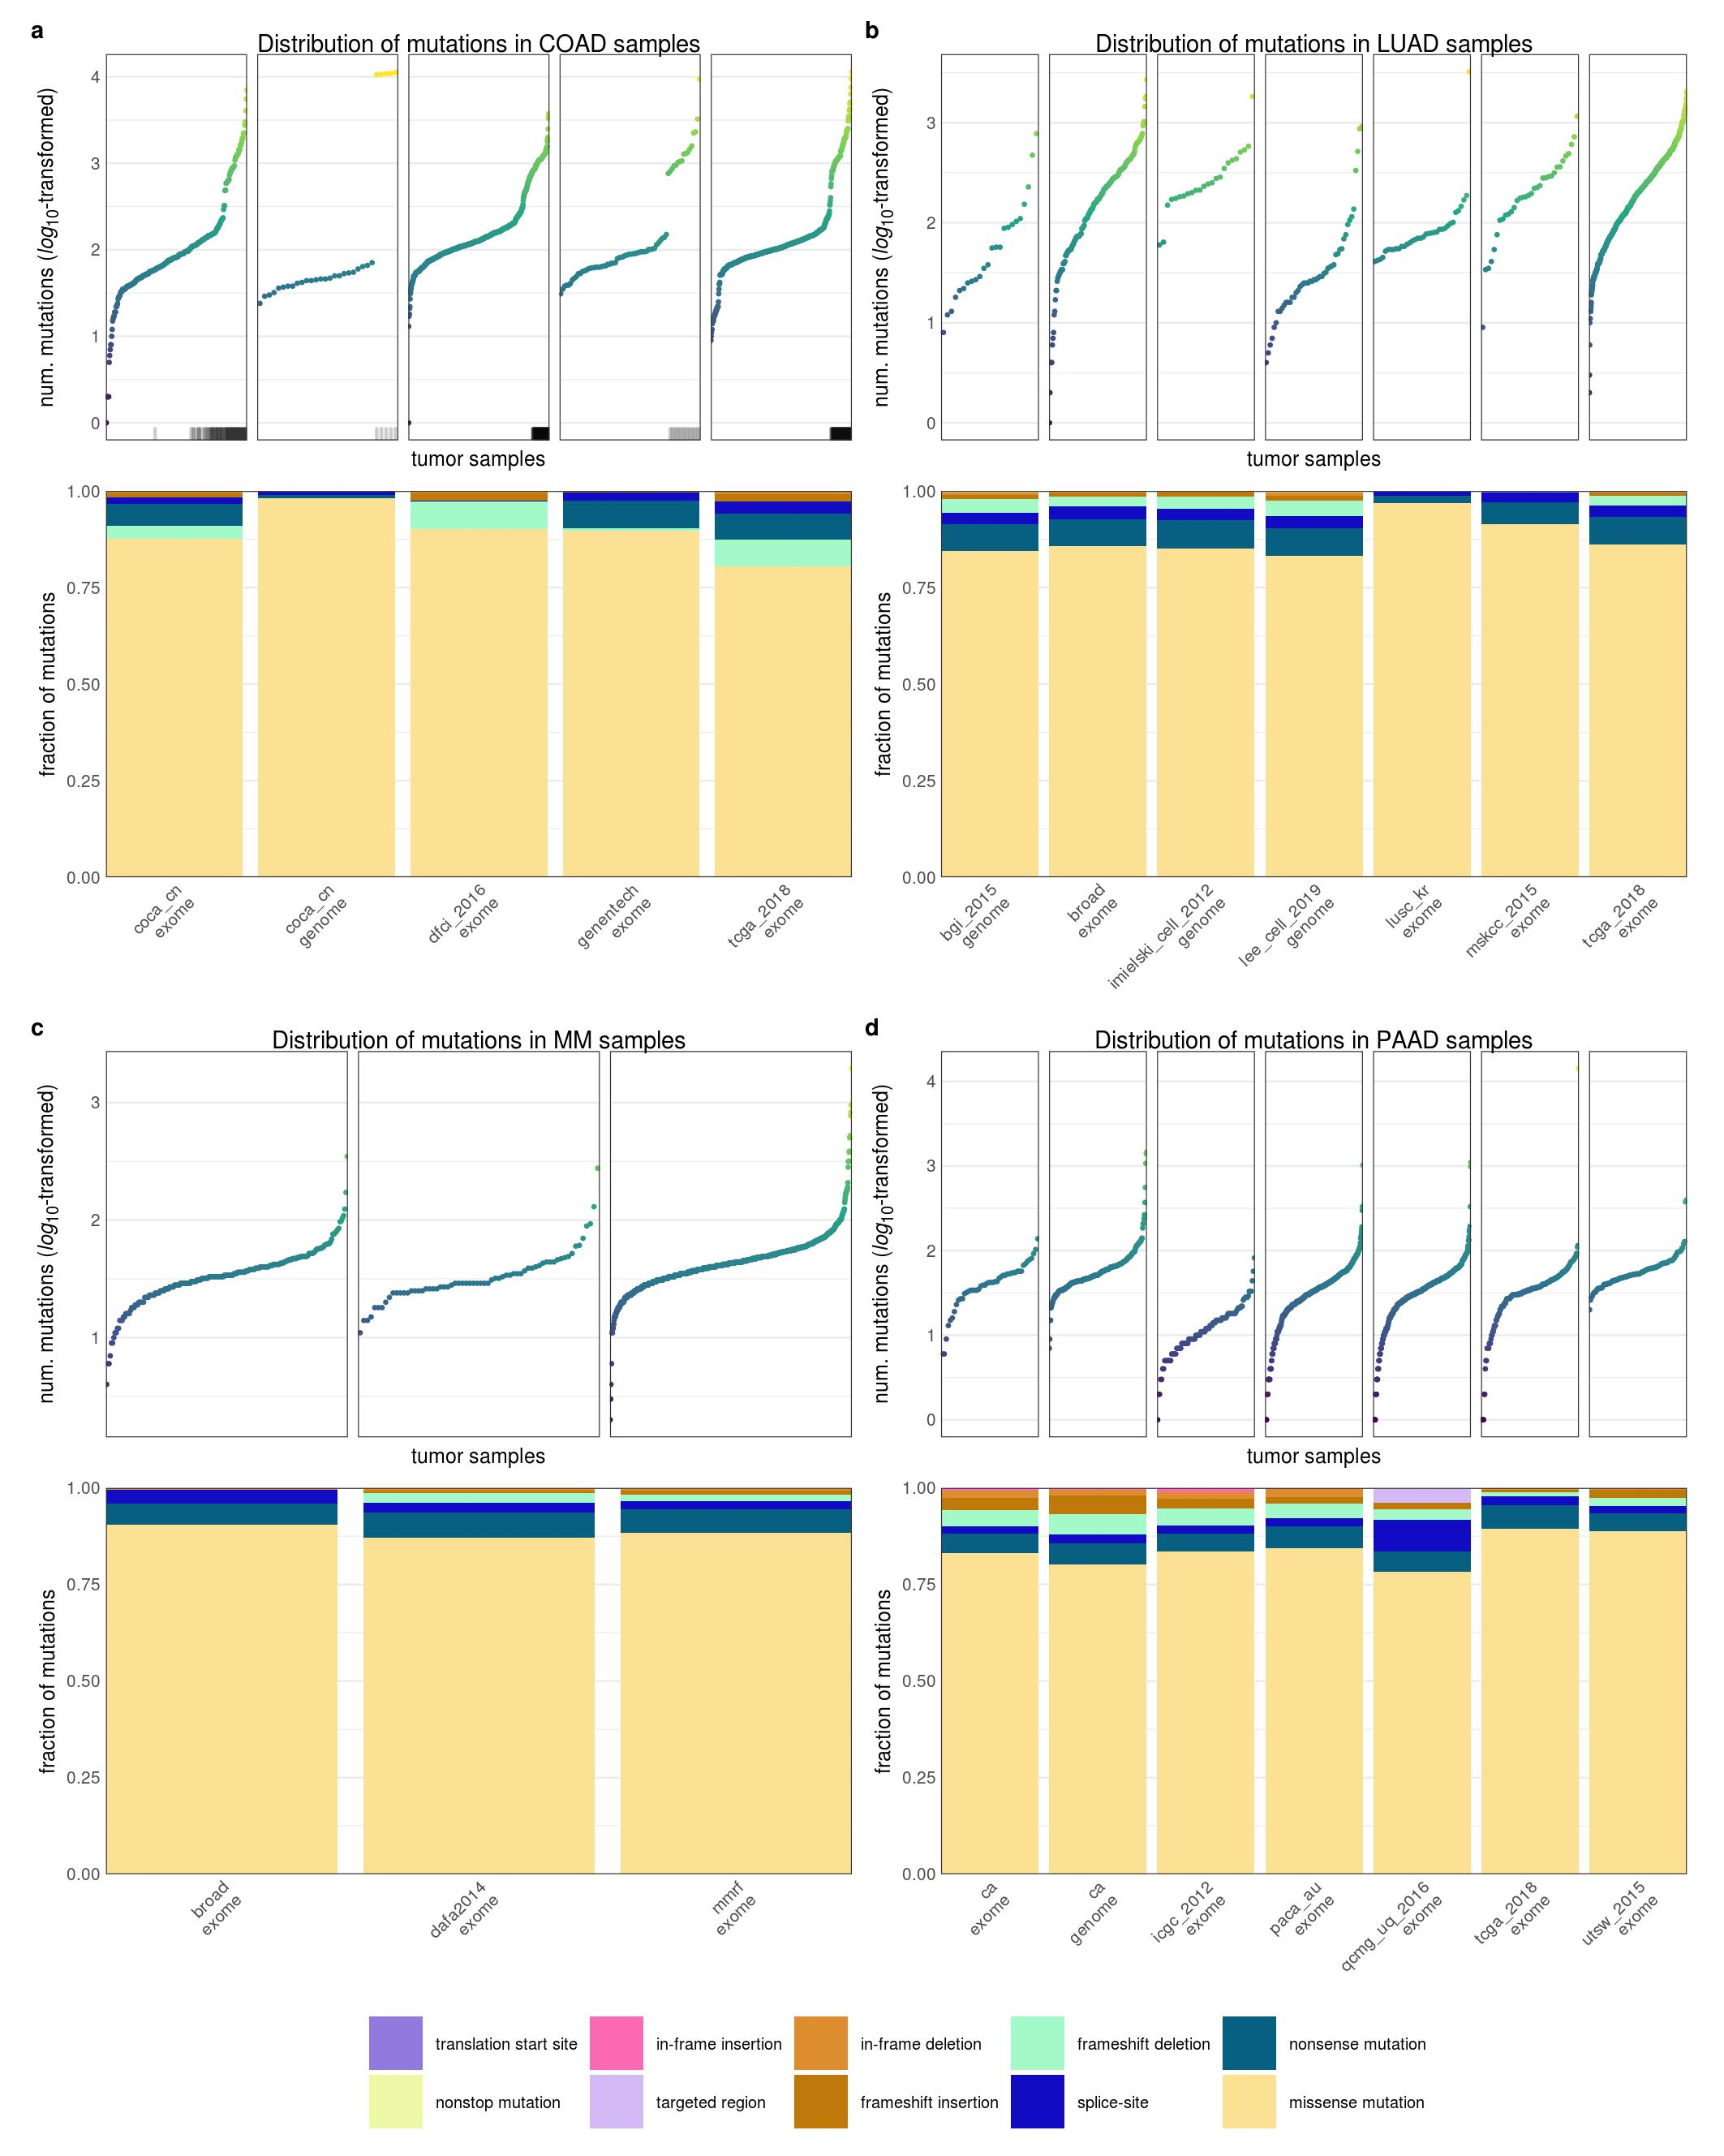
\includegraphics[height=150mm]{figures/SuppFigure_04.jpeg}
\caption{
    \textbf{The mutation burden and types of mutations of coding regions in human cancer samples.}
    \textbf{a-d.} The number of coding mutations per sample are shown as scatter plots with the samples arranged in order of increasing mutational burden (top) followed by the distribution of the types of mutations (bottom). The samples were separated by type of cancer and by source of the sequencing data.
    For COAD (\textbf{a}), the location of MSI-H and hypermutants are indicated by the tick marks along the x-axis of the scatter plot.
}
\label{sfig:mutation-burden-of-cancer-samples}
\end{figure}


\begin{figure}
\centering
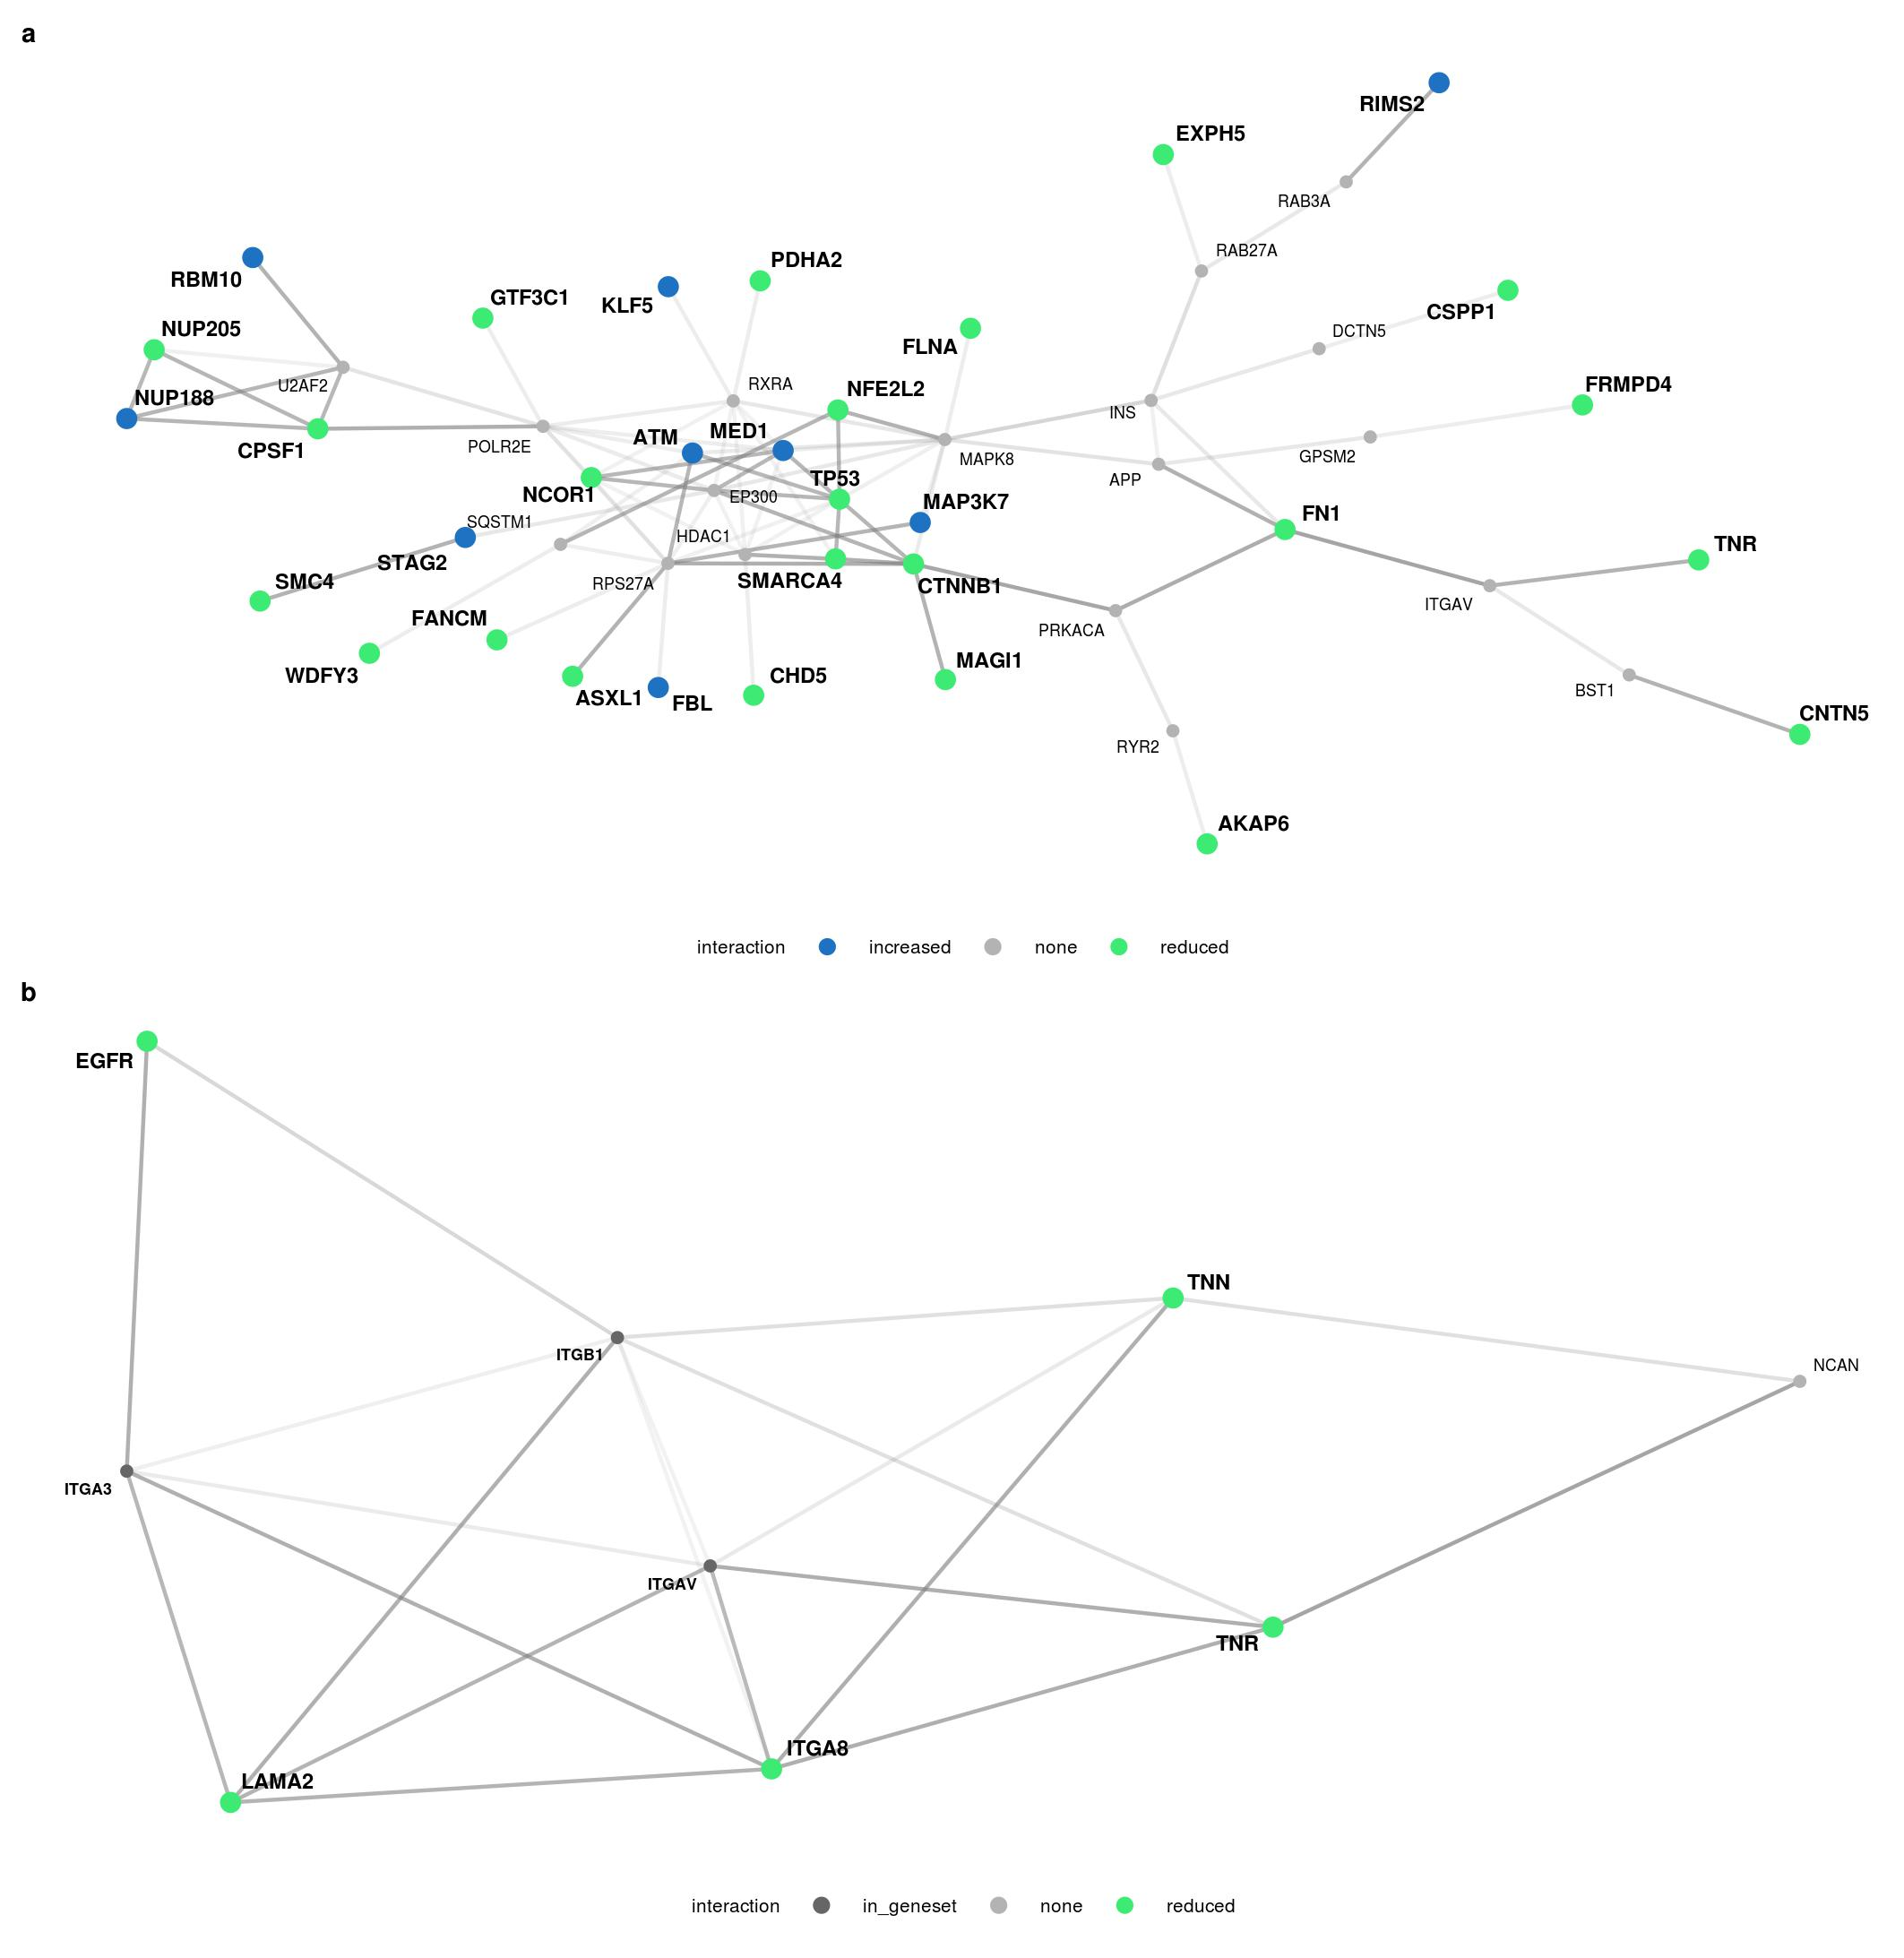
\includegraphics[height=170mm]{figures/SuppFigure_11.jpeg}
\caption{
    \textbf{The survival curves of patients with LUAD stratified by \KRAS{} mutation and protein-protein interactions (PPI) of enriched functions in the \KRAS{} allele comutation networks in LUAD.}
    \textbf{a-c.} Survival curves of LUAD patients stratified by (\textbf{a}) \KRAS{} WT or mutant, (\textbf{b}) \KRAS{} allele, and (\textbf{c}) only \KRAS{} WT and \KRAS{} G12C. Each survival curve is labeled with the p-value from either the (\textbf{a, c}) log-rank test or (\textbf{b}) likelihood ratio test.
    \textbf{d.} The PPI of the transcription factor Myc that was detected to comutate with \KRAS{} G12C in LUAD.
    \textbf{e.} The subnetwork of the focal adhesion PPI that was detected to comutate with \KRAS{} G12D in LUAD.
    For both subnetworks, the nodes represent proteins and edges represent physical PPI. Colored nodes had a comutation interaction with the respective \KRAS{} allele, the color indicating whether it was a reduced (green) or increased (blue) rate of comutation.
    The bold protein names indicate that the gene was included in the enriched gene set.
    Edge thickness is related to the centrality of the interaction to the presented subnetwork.
}
\label{sfig:luad-comutation-supplementary}
\end{figure}


\begin{figure}[p]
\centering
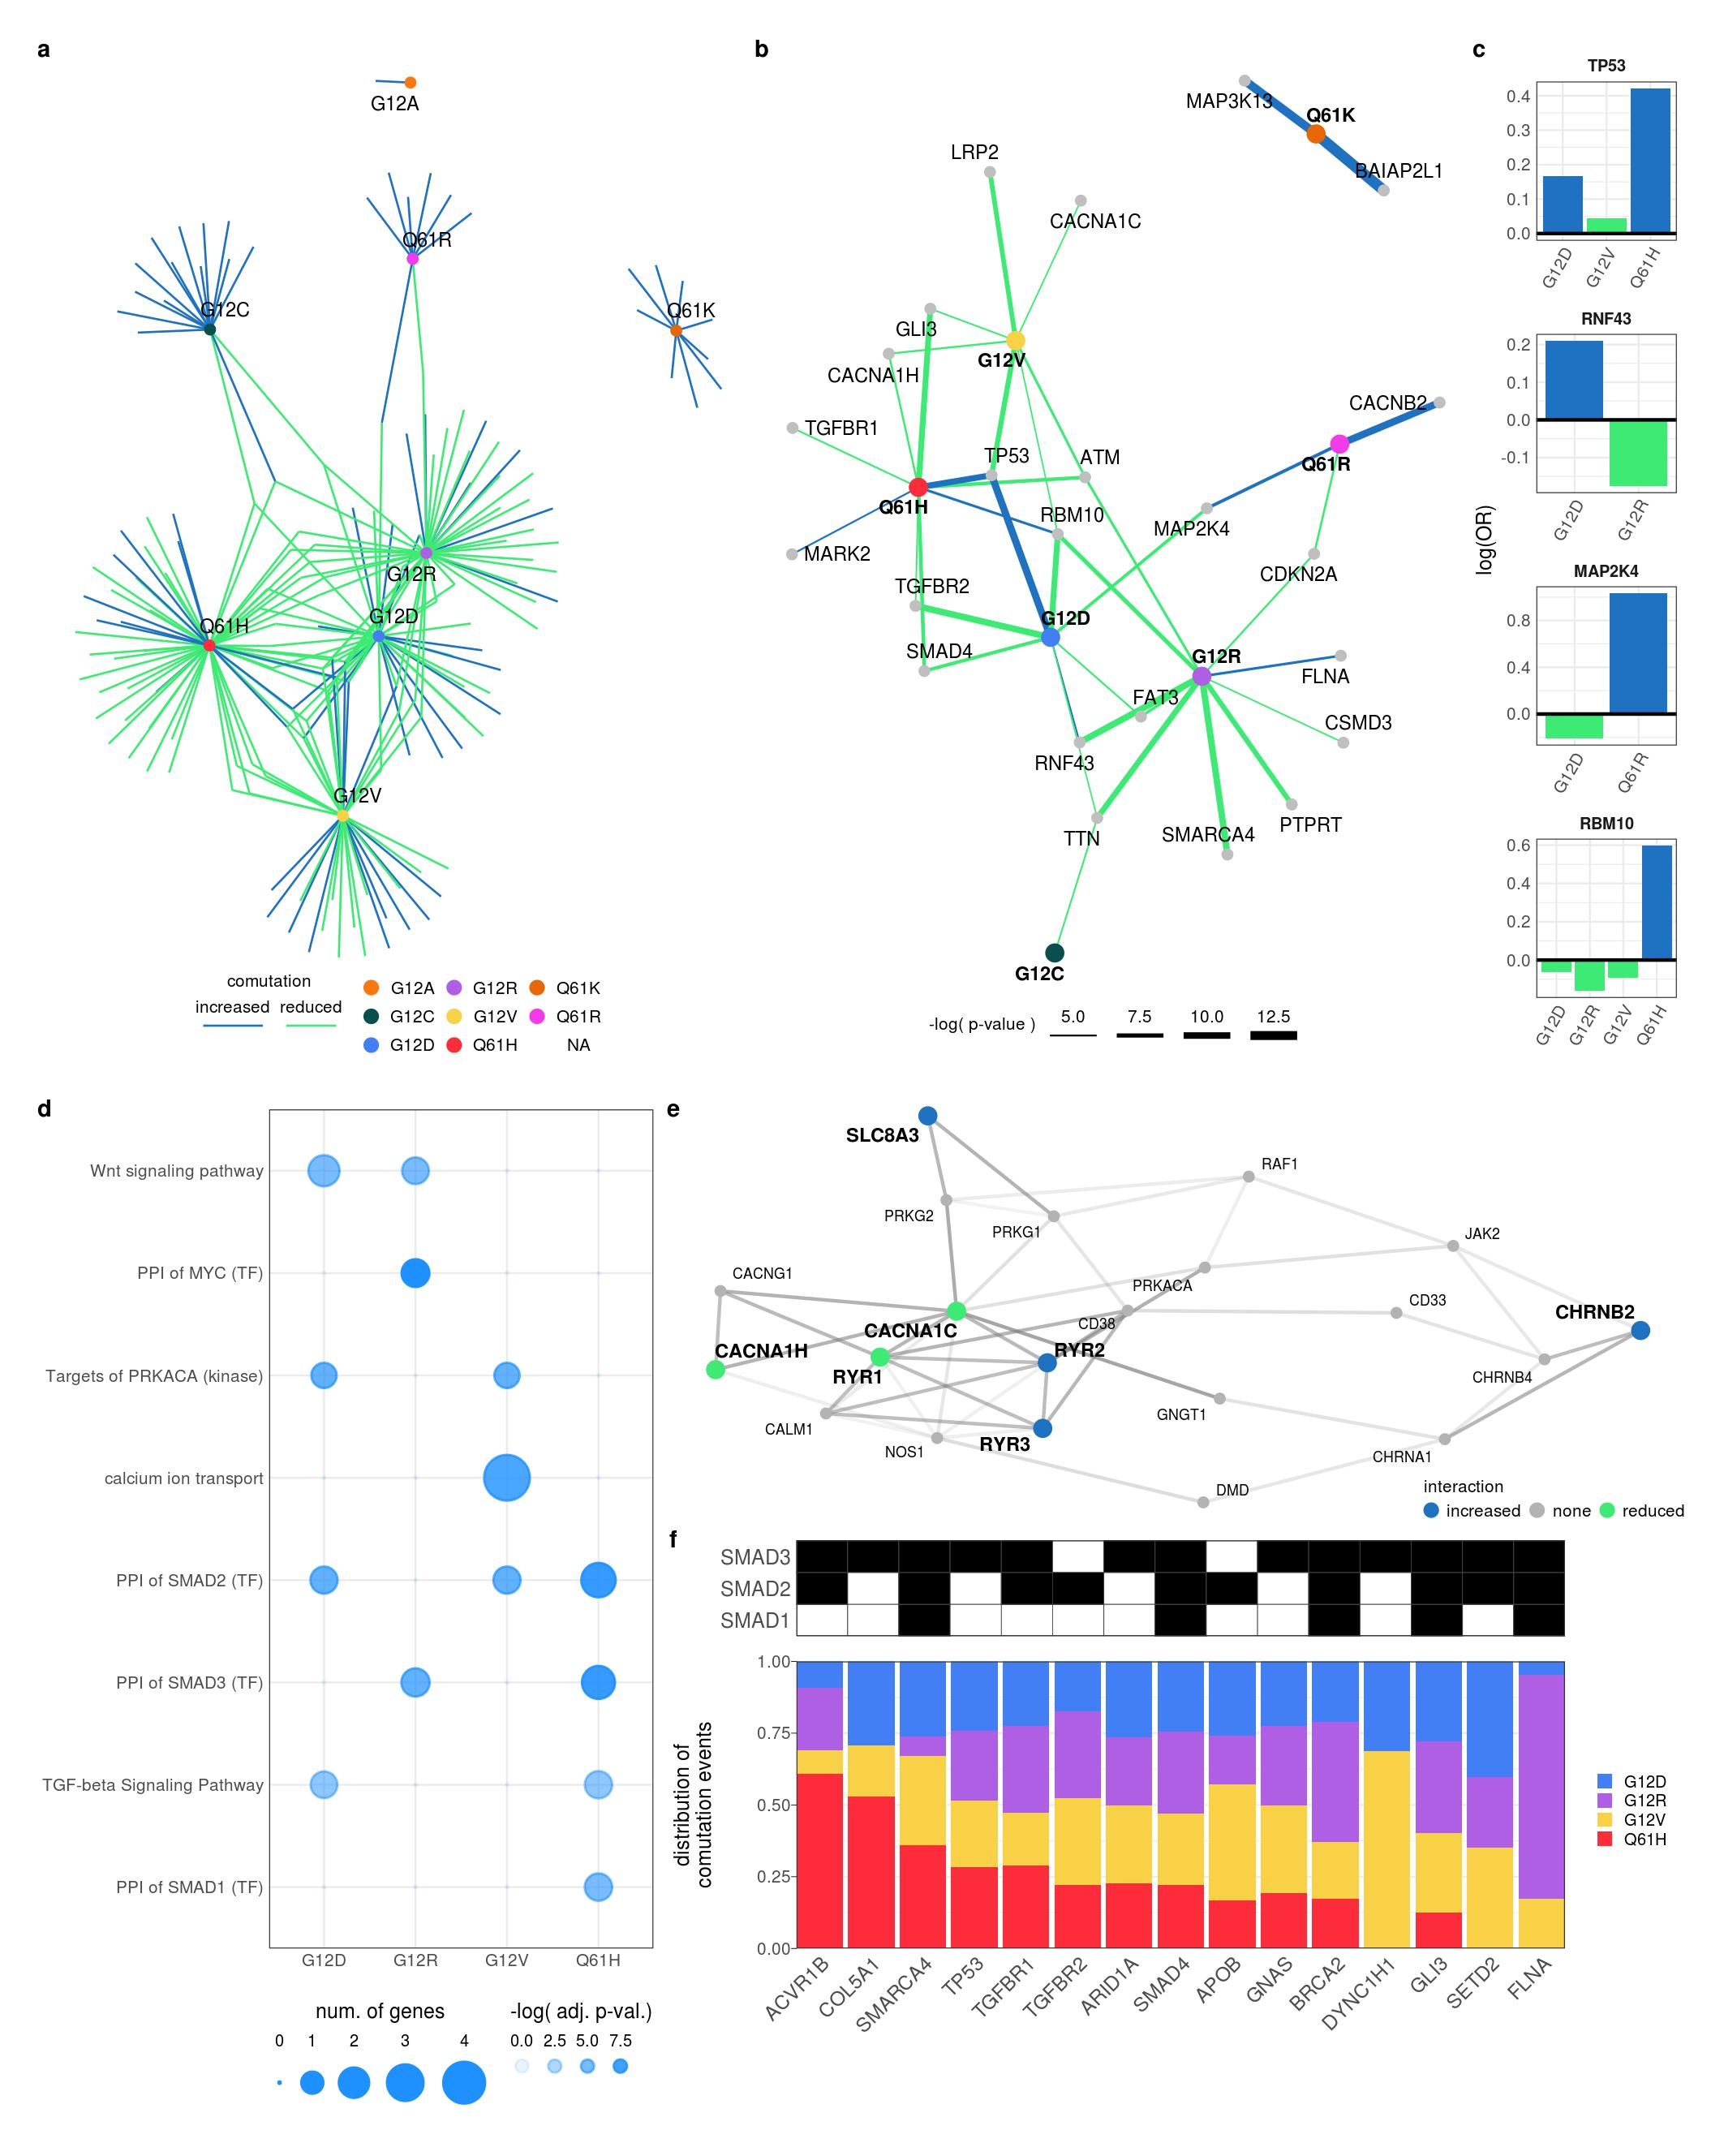
\includegraphics[height=110mm]{figures/SuppFigure_12.jpeg}
\caption{
    \textbf{The comutation networks of common \KRAS{} alleles in PAAD.}
    \textbf{a.} The comutation network of the \KRAS{} alleles in PAAD where each edge represents a comutation interaction between an allele and another gene. The color of the edge indicates whether the interaction was an increase (blue) or decrease (green) in the frequency of comutation.
    \textbf{b.} A subset of the network shown in \textbf{a} of genes known to physically interact with \KRAS{}, are in one of its canonical up- or downstream pathways, or are validated oncogenes. The width of the edge indicates the strength of the association.
    \textbf{c.} The log-odds of comutation between \KRAS{} alleles and other genes that had detectable opposing comutation interactions with multiple alleles.
    \textbf{d.} Cellular functions enriched in the comutation networks of the \KRAS{} alleles. The size of the dot indicates the number of genes in both the function and the comutation network, and the transparency indicates the strength of the association.
    \textbf{e.} The PPIN of proteins encoded by the genes constituting the "calcium ion transport" enriched in the comutation network of \KRAS{} G12V. The colored nodes indicate the genes in the comutation network, the color indicating the type of comutation interaction between the gene and G12V. The grey nodes were selected as they were most central to connecting the highlighted genes.
    \textbf{f.} A comparison of the comutation rates of the genes producing proteins in the PPI of SMAD1-3. Each column is a gene with a comutation interaction with a \KRAS{} allele and in at least one of the gene sets. The black tiles on top indicate that the gene was in the PPI of the indicated SMAD protein. The bar plot shows the distribution of the comutation events of each gene across tumor samples with the various \KRAS{} mutations.
}
\label{sfig:paad-comutation}
\end{figure}


\begin{figure}[p]
\centering
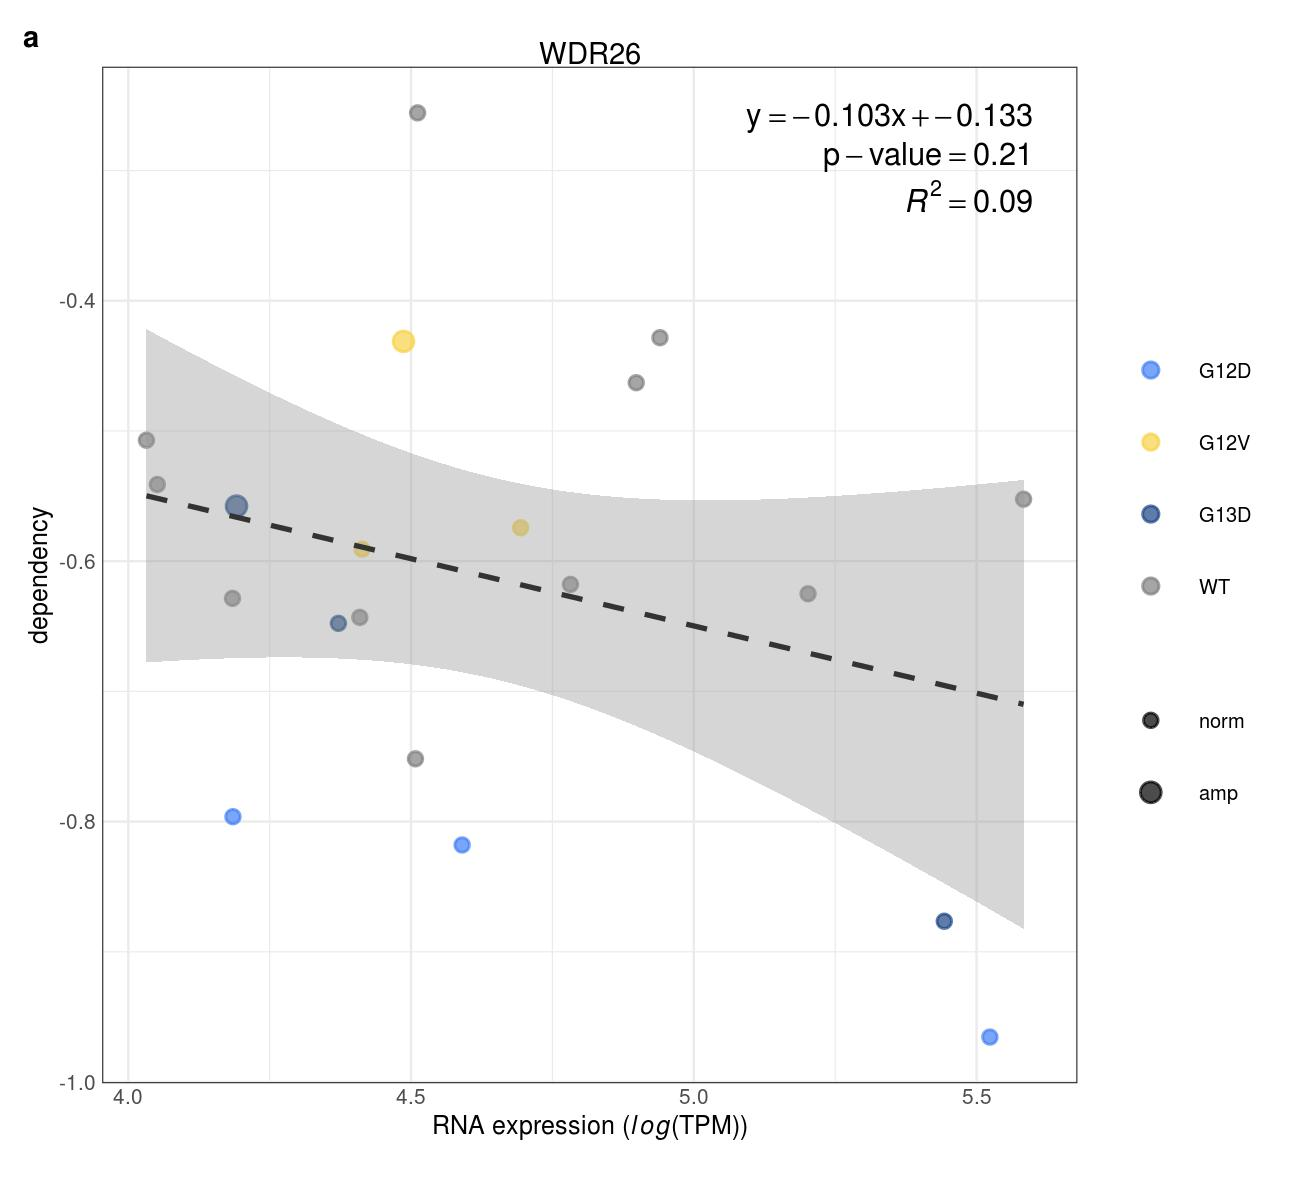
\includegraphics[height=100mm]{figures/SuppFigure_15.jpeg}
\caption{
    \textbf{Association between \emph{WDR26} RNA expression and dependency score in COAD cell lines.}
    \textbf{a.} The dependency score of knocking out \emph{WDR26} against the gene's RNA expression (log-transformed TPM with a pseudocount of 1). Each point represents a COAD cell line, colored by the \KRAS{} allele. The size of the point represents the copy number of \emph{WDR26} where "norm" is 2 copies and "amp" is amplified. The dashed line represents the line-of-best fit. The equation, p-value, and $R^2$ for the line are shown in the top-right.
}
\label{sfig:coad_dep_wdr26}
\end{figure}


\begin{figure}
\centering
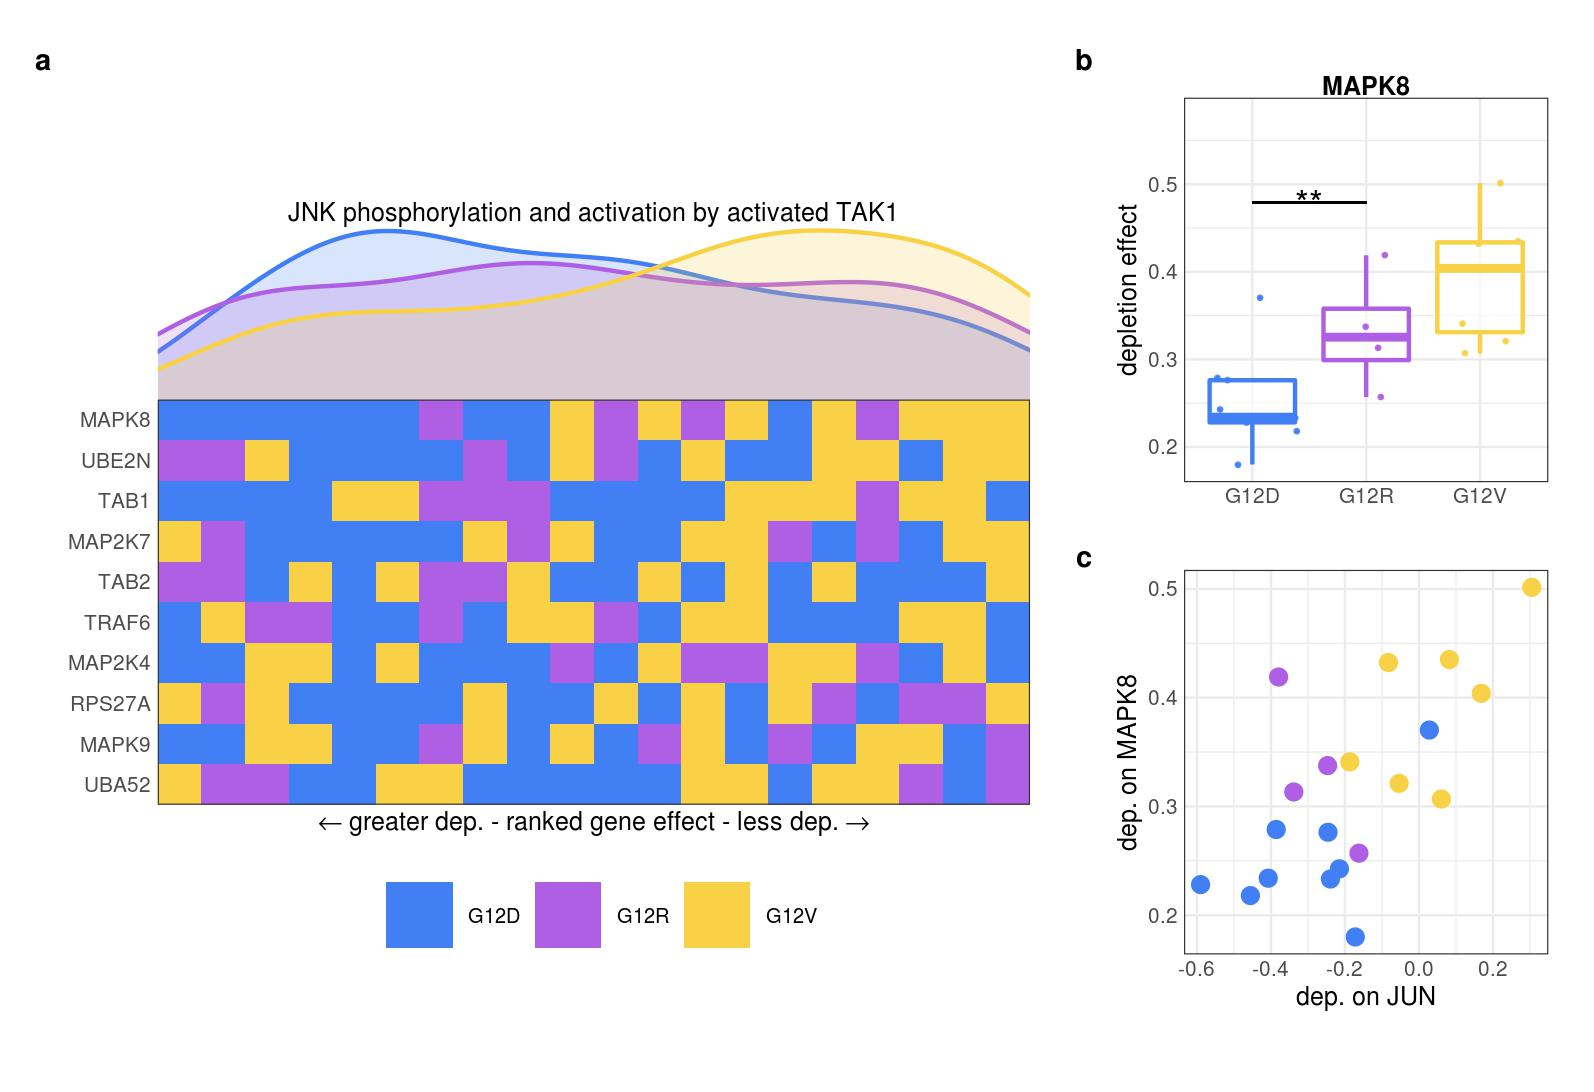
\includegraphics[width=\textwidth]{figures/SuppFigure_14.jpeg}
\caption{
    \textbf{Reduced dependency on JNK signaling in PAAD cell lines with \KRAS{} G12V mutations.}
    \textbf{a.} The "JNK phosphorylation and activation by activated TAK1" gene set was significantly enriched for reduced genetic dependency in PAAD cell lines with \KRAS{} G12V. Each row represents a gene and each cell represents a cell line colored by its \KRAS{} allele. The cell lines were arranged in ranking order by their dependency score for each gene. Thus, each column indicates a rank. The line plots above the heatmap indicate the representation (density) of each \KRAS{} allele at each rank across the genes.
    \textbf{b.} The genetic dependency on \emph{MAPK8} of cell lines of different \KRAS{} alleles in PAAD (**: p < 0.01; p-values were adjusted using the Benjamini-Hochberg FDR correction method).
    \textbf{c.} The genetic dependency on \emph{JUN} and \emph{MAPK8} of cell lines of different \KRAS{} alleles in PAAD. Each point is a cell line colored according to its \KRAS{} allele. The dashed line represents the line-of-best fit. The equation, p-value, and $R^2$ for the line are shown in the top-right.
}
\label{sfig:paad-dependency-JUN}
\end{figure}


\end{document}
